\chapter{Implementasi dan Pengujian}
\label{chap:implementasi dan pengujian}

Pada bab ini akan dibahas mengenai implementasi dari antarmuka perangkat lunak, dan pengujian perangkat lunak di \textit{workspace} tempat program ini diregistrasikan beserta pengujian eksperimental perangkat lunak di \textit{workspace} lain dari \textit{Slack}.

\section{Implementasi}
 Untuk mengimplementasi perangkat lunak ini, langkah awal yang dikerjakan adalah mencoba membuat program yang awalnya berjalan di \textit{localhost}. Setelah berjalan dan berhasil di \textit{localhost}, maka langkah selanjutnya yaitu membuat akun \textit{Heroku} lalu membuat sebuah aplikasi baru yang berbasis \textit{Node.js} serta melakukan \textit{deploy} kode perangkat lunak yang sudah berhasil berjalan di \textit{localhost} ke \textit{Heroku}. Aplikasi yang dibuat di \textit{Heroku} diberi nama \textit{slack-status-changer} dan dapat diakses dengan cara membuka \url{https://slack-status-changer.herokuapp.com/}. Setelah melakukan \textit{deploy} ke dalam \textit{Heroku}, maka perangkat lunak juga dilakukan pengujian agar fungsi yang sudah berjalan pada saat di \textit{localhost} masih bisa berjalan semua pada saat setelah perangkat lunak dimasukkan ke dalam \textit{Heroku}. Lalu setelah semua berjalan dengan sesuai fungsinya, maka langkah yang dilakukan selanjutnya adalah memasukkan sebuah \textit{job} pada \textit{Heroku Scheduler} untuk \textit{scheduler} menjalankan \textit{job} itu sesuai iterasi waktunya yaitu per 10 menit sekali. 
 
\subsection{Lingkungan Pengembangan}
 Pada subbab ini akan disebutkan spesifikasi perangkat keras maupun perangkat lunak yang dipakai untuk menyusun skripsi ini:
\subsubsection{Spesifikasi Perangkat Keras}
\begin{itemize}
    \item Processor Intel® Core™ i5-8250U CPU @ 1.60GHz × 8 
    \item Graphics Intel® UHD Graphics 620 \(Kabylake GT2\)
    \item RAM 12 GB
    \item Harddisk 1000GB HDD
\end{itemize}
\subsubsection{Spesifikasi Perangkat Lunak}
\begin{itemize}
    \item Sistem Operasi Ubuntu 18.04.3 LTS 64-bit
    \item Atom
    \item Node.js version 8.10.0
    \item NPM version 6.8.0
    \item pgAdmin4 version 4.13 (Application Mode: Desktop)
\end{itemize}

\subsection{Implementasi Basis Data}
Untuk basis data yang diimplementasikan, tabel yang disediakan hanya ada 1 tabel yang bernama \textit{Credentials}. Tabel basis data ini menampung data-data kredensial dari pengguna yang menjalankan dan mendaftarkan akunnya ke program ini. Tabel ini dibuat dengan bantuan \textit{pgAdmin4} yang melakukan koneksi kepada \textit{url} yang diberikan \textit{Heroku Postgres} sehingga tabel ini disimpan pada \textit{Heroku Postgres} yang bersangkutan dengan perangkat lunak yang di \textit{deploy} ke \textit{Heroku}. 

\subsection{Implementasi Antarmuka}
Hasil implementasi dari antarmuka perangkat lunak ini dapat dilihat pada gambar \ref{fig:antarmuka_awal}, gambar \ref{fig:login_win_live}, gambar \ref{fig:izin_win_live}, gambar \ref{fig:petunjuk_login_slack}, gambar \ref{fig:login_slack}, gambar \ref{fig:izin_slack}, dan gambar \ref{fig:setelah_selesai}. 

\begin{figure}[h]
  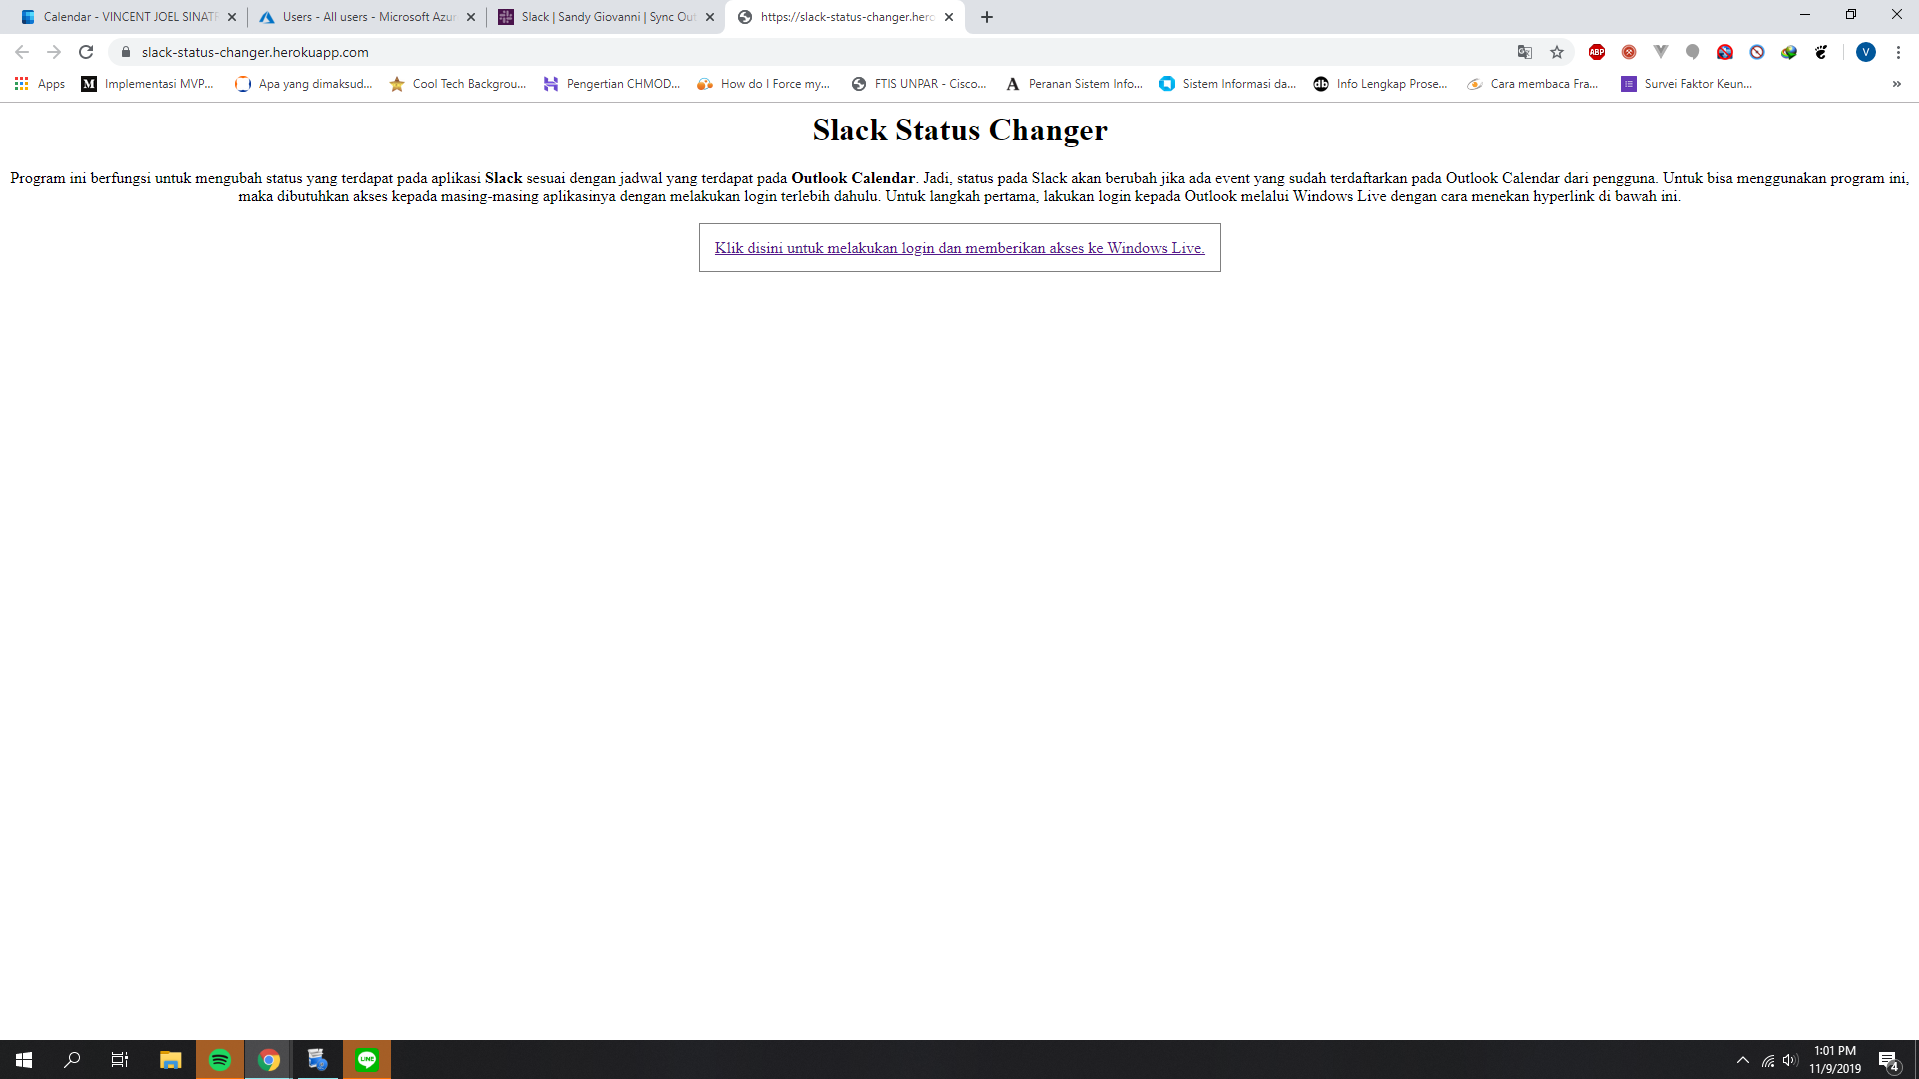
\includegraphics[width=10cm]{./Gambar/Step1.png}
  \centering
  \caption{Antarmuka halaman awal.}
  \label{fig:antarmuka_awal}
\end{figure}

\begin{figure}[h]
  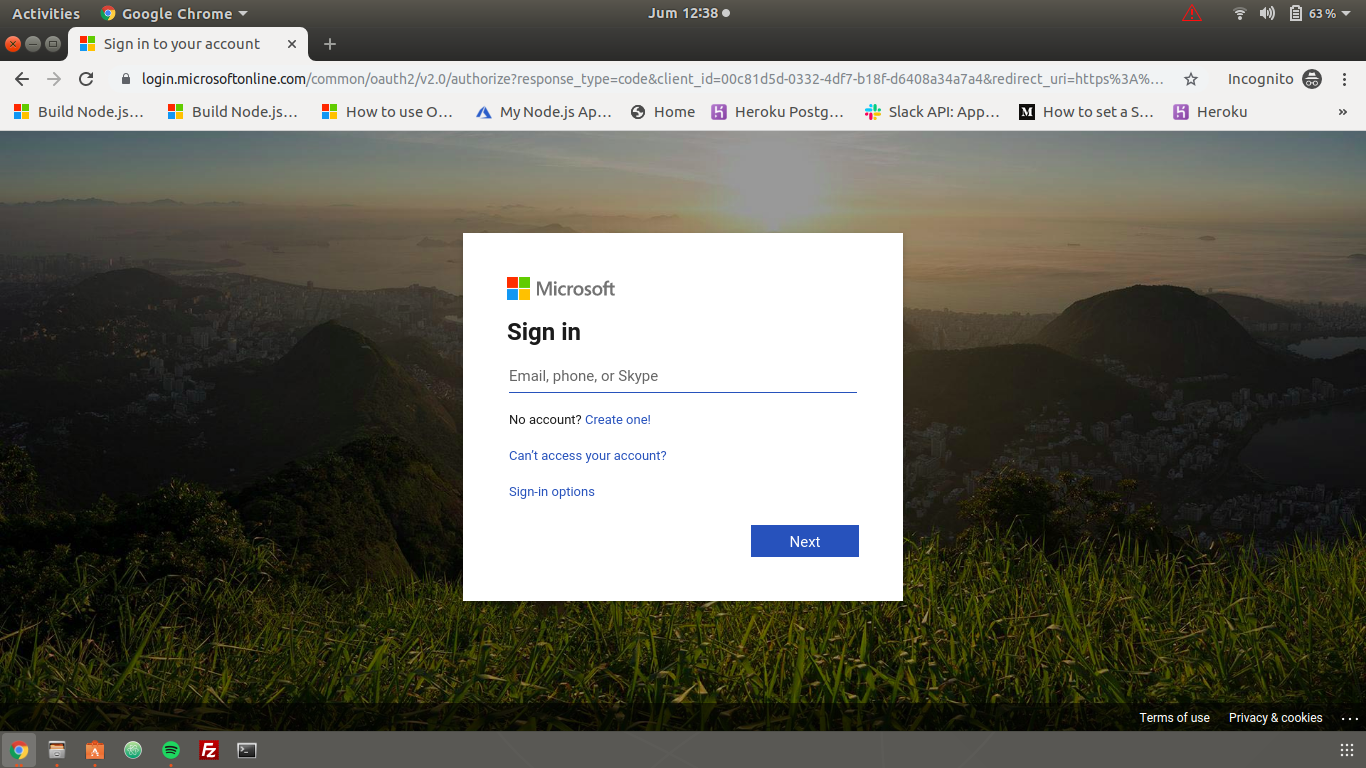
\includegraphics[width=10cm]{./Gambar/Step2.png}
  \centering
  \caption{Antarmuka untuk login Windows Live.}
  \label{fig:login_win_live}
\end{figure}

\begin{figure}[h]
  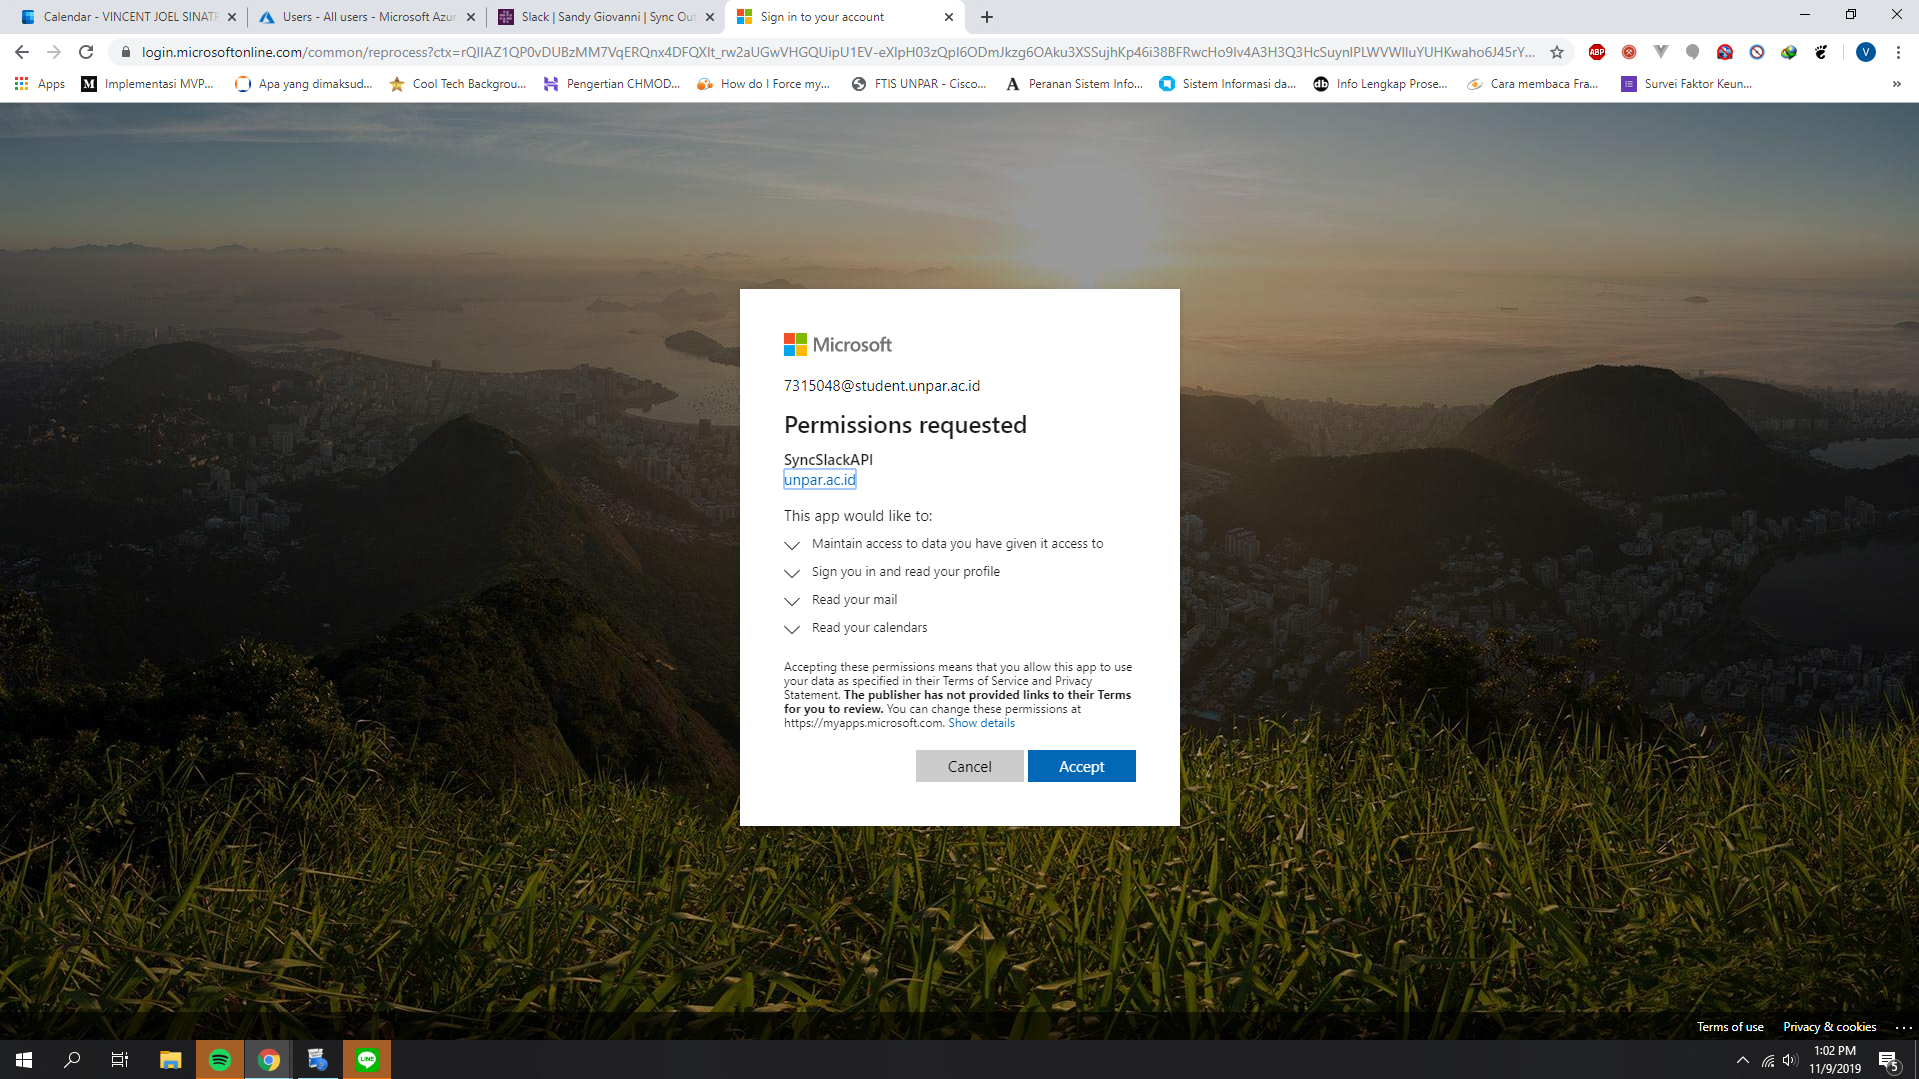
\includegraphics[width=10cm]{./Gambar/Step3.png}
  \centering
  \caption{Antarmuka untuk memberikan Windows Live izin ke perangkat lunak.}
  \label{fig:izin_win_live}
\end{figure}

\begin{figure}[h]
  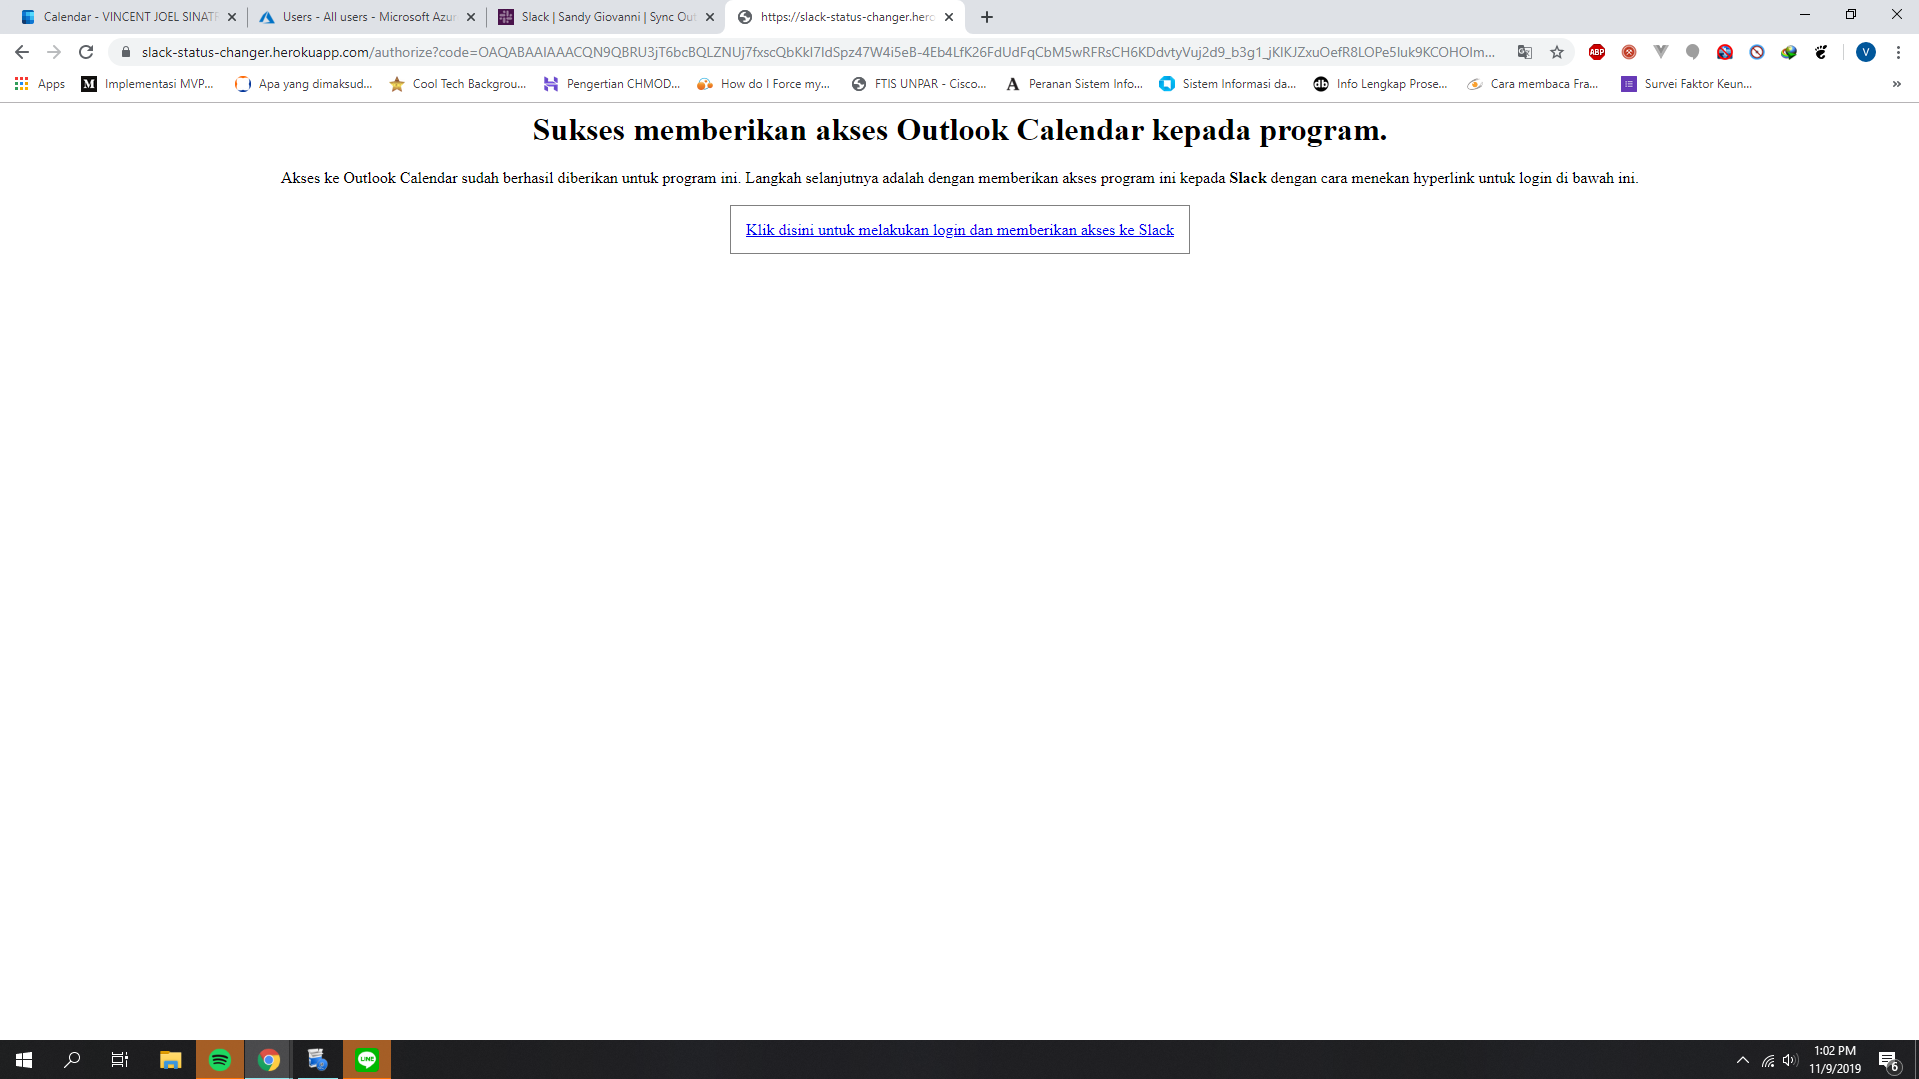
\includegraphics[width=10cm]{./Gambar/Step4.png}
  \centering
  \caption{Antarmuka petunjuk login ke Slack.}
  \label{fig:petunjuk_login_slack}
\end{figure}

\begin{figure}[h]
  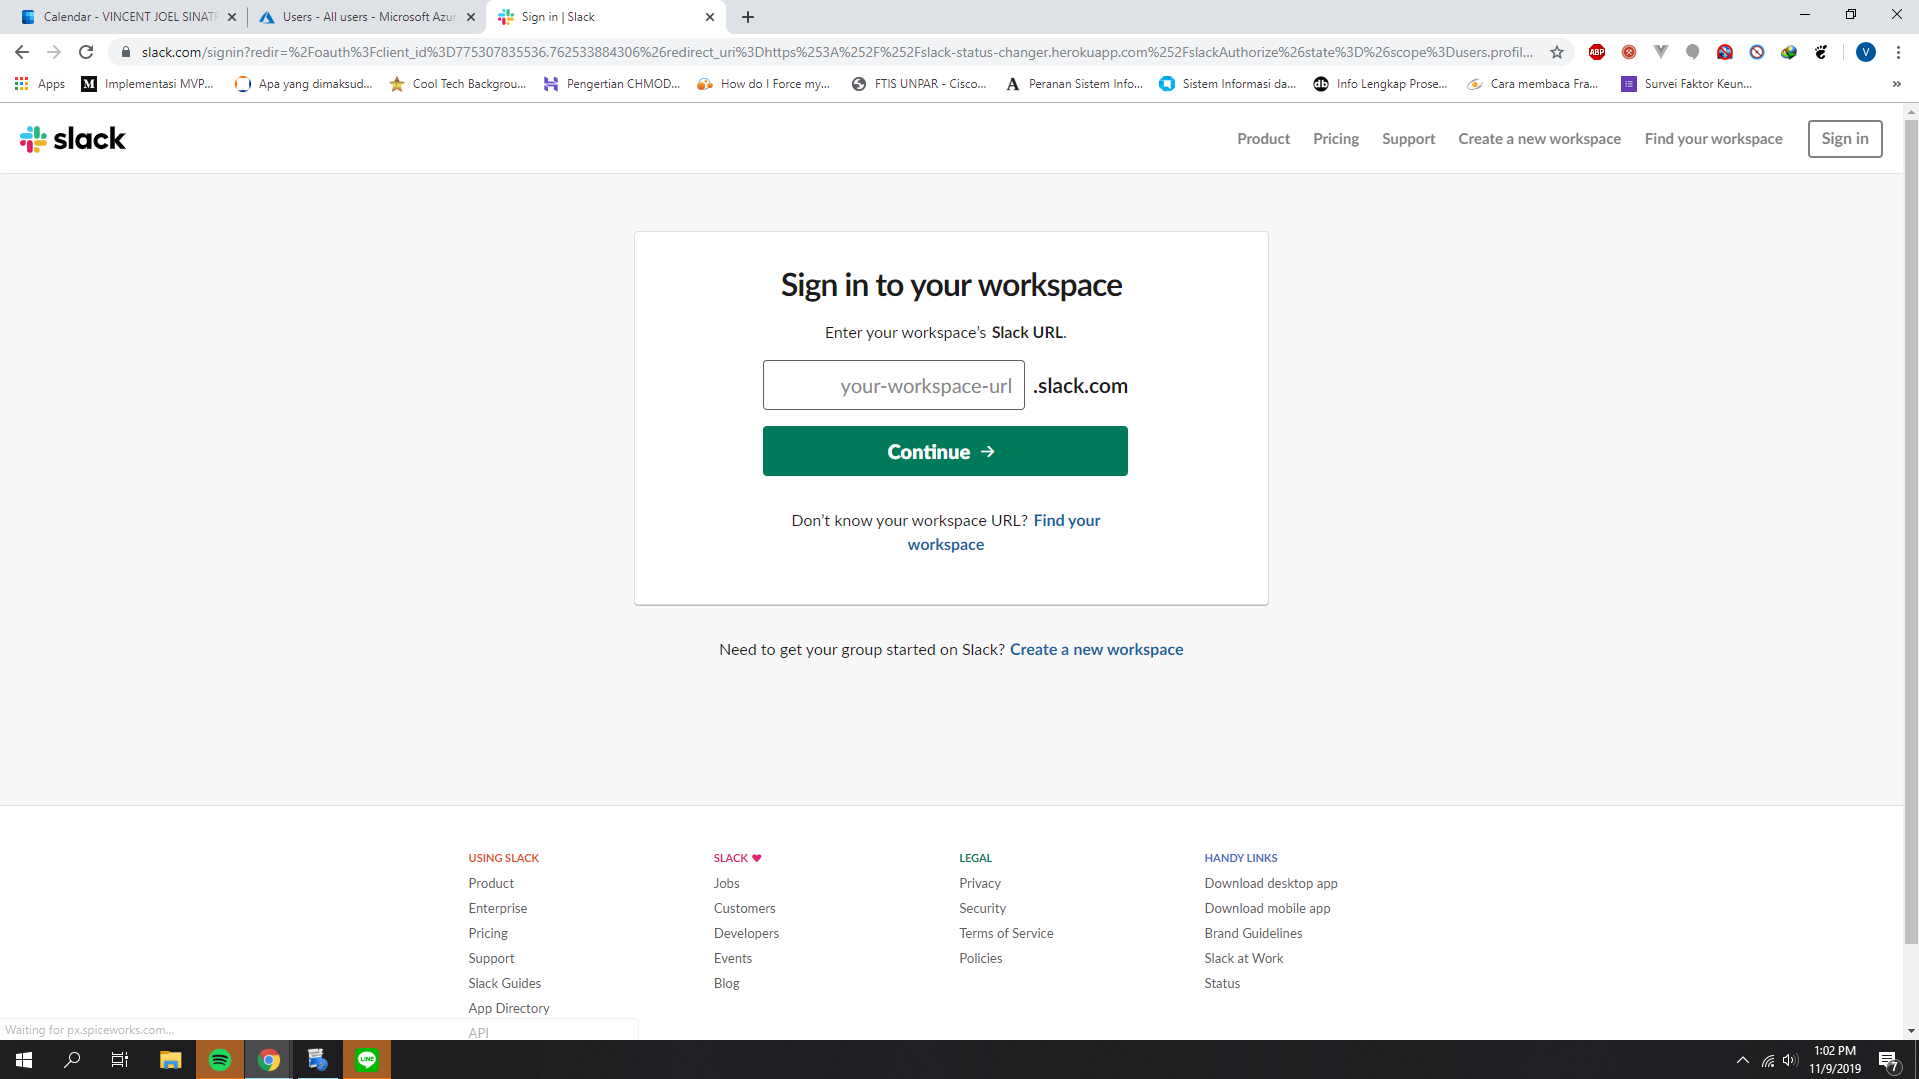
\includegraphics[width=10cm]{./Gambar/Step5.png}
  \centering
  \caption{Antarmuka untuk login Slack.}
  \label{fig:login_slack}
\end{figure}

\begin{figure}[h]
  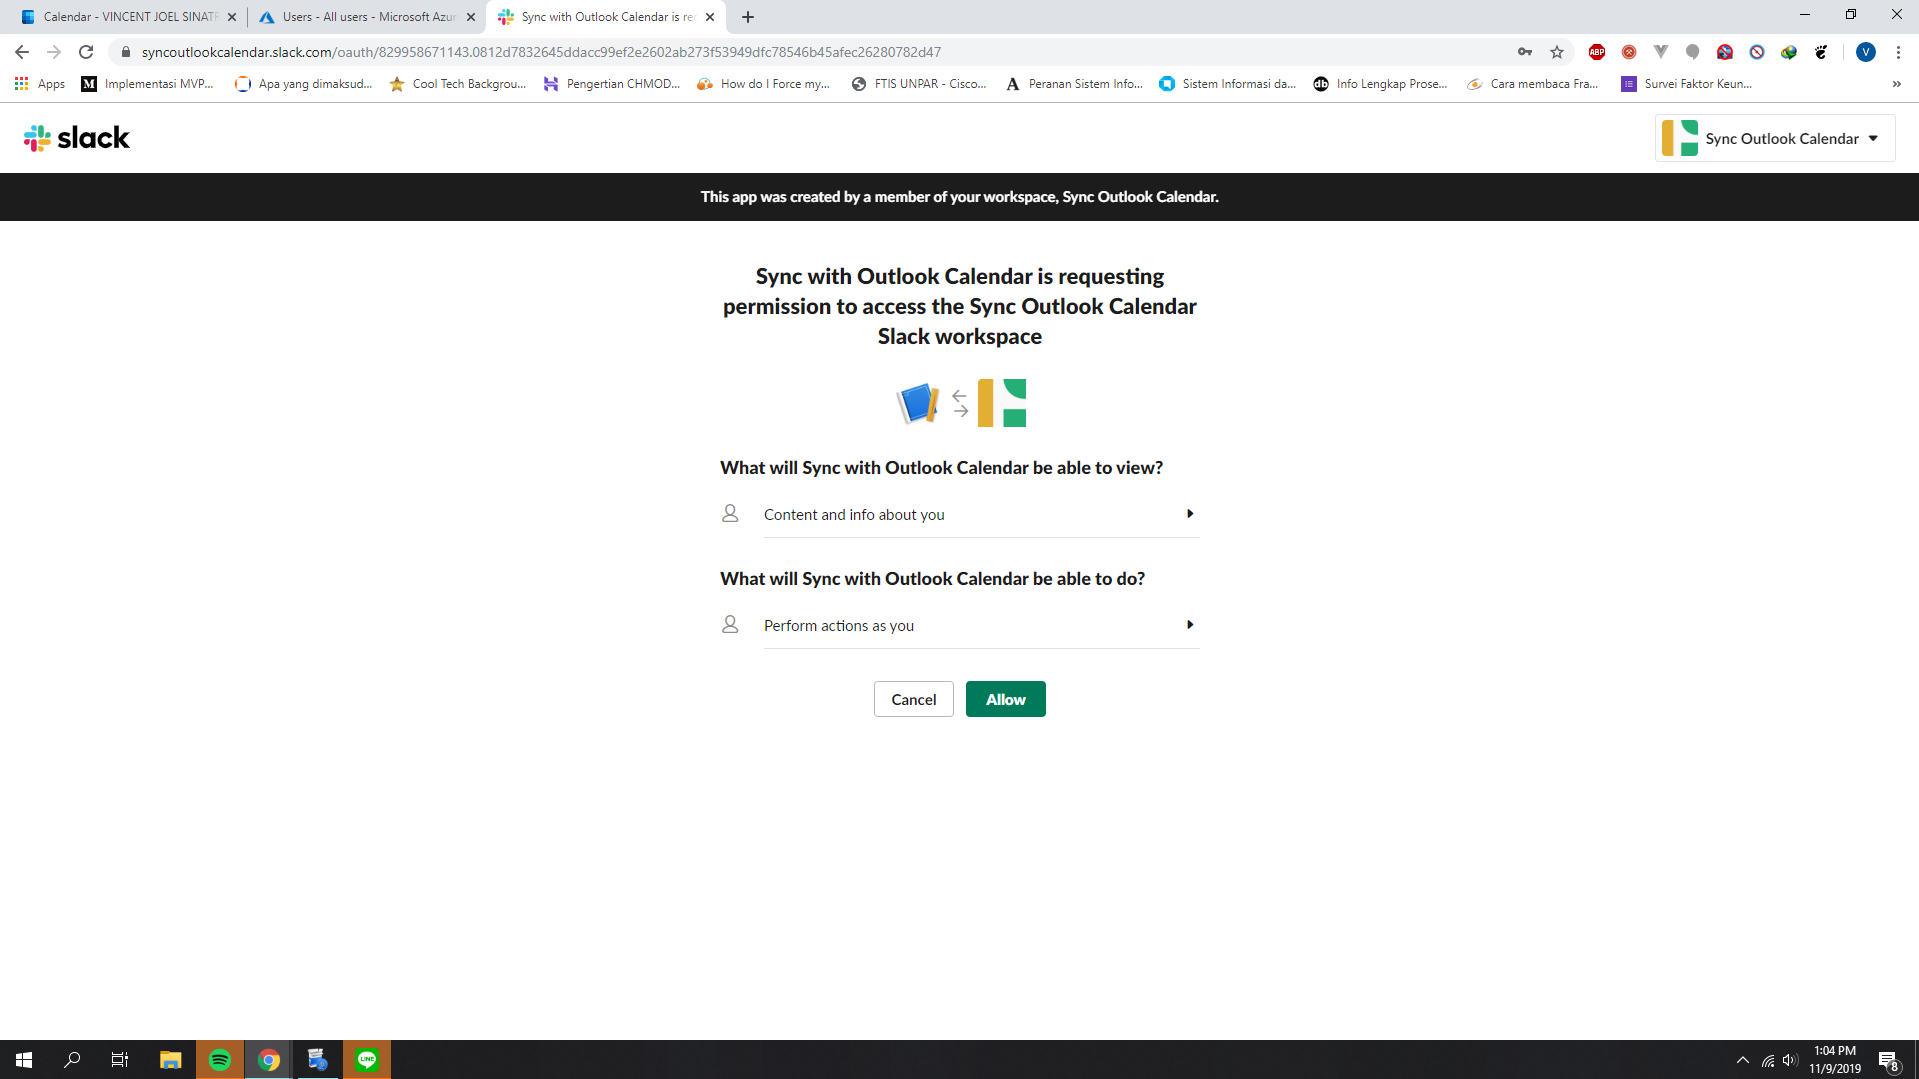
\includegraphics[width=10cm]{./Gambar/Step6.png}
  \centering
  \caption{Antarmuka untuk memberikan Slack izin ke perangkat lunak.}
  \label{fig:izin_slack}
\end{figure}

\begin{figure}[h]
  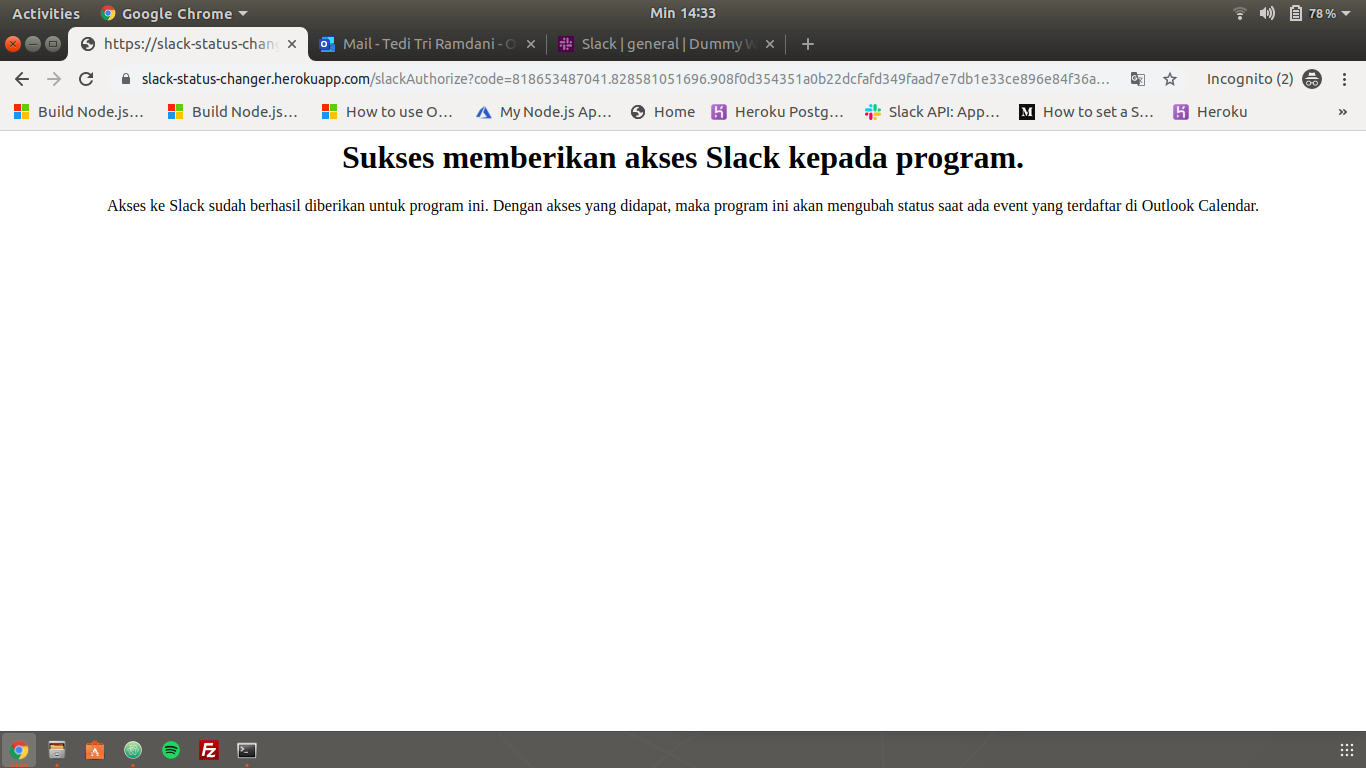
\includegraphics[width=10cm]{./Gambar/Step7.png}
  \centering
  \caption{Antarmuka saat selesai melakukan login dan pemberian izin.}
  \label{fig:setelah_selesai}
\end{figure}
\clearpage

Pada gambar \ref{fig:antarmuka_awal} merupakan tampilan awal yang berisikan penjelasan dari perangkat lunak ini untuk dapat dipahami oleh pengguna serta sebuah tombol yang membawa pengguna masuk ke halaman \textit{login Windows Live} seperti pada gambar \ref{fig:login_win_live}. Setelah \textit{login}, maka akan muncul tampilan seperti gambar \ref{fig:izin_win_live} untuk perangkat lunak meminta izin kepada pengguna untuk perangkat lunak mengakses dan mendapatkan informasi data \textit{event} di dalam \textit{Outlook Calendar}. 

Setelah berhasil melakukan \textit{login} dan pengguna memberikan izin akses kepada perangkat lunak ini, maka akan tampil tampilan seperti tampilan gambar \ref{fig:petunjuk_login_slack} yang berisi penjelasan akan langkah selanjutnya yang perlu dilakukan pengguna untuk bisa memakai perangkat lunak ini dan juga ada satu tombol yang mengarahkan pengguna melakukan langkah yaitu melakukan \textit{login} seperti pada gambar \ref{fig:login_slack}. Setelah berhasil melakukan \textit{login}, maka akan muncul tampilan untuk meminta izin dari pengguna \textit{Slack} kepada perangkat lunak seperti pada gambar \ref{fig:izin_slack}. 

Setelah pengguna berhasil \textit{login} dan memberikan akses kepada perangkat lunak maka akan ditampilkan halaman seperti gambar \ref{fig:setelah_selesai}. 

\section{Hasil Implementasi}
Hasil implementasi dari perangkat lunak ini berupa kode program yang dibangun dengan menggunakan bahasa pemrograman \textit{Node.js} dengan aplikasi \textit{Atom} sebagai \textit{text editor} dan juga \textit{pgAdmin4} sebagai aplikasi yang menghubungkan dengan basis data dari \textit{Heroku Postgres}.  

\section{Pengujian}
Pada bagian pengujian, akan dibagi kepada 2 tipe pengujian yaitu pengujian fungsional dan juga pengujian eksperimental. Pada pengujian fungsional, akan dicoba tombol-tombol sesuai dengan fungsinya dan juga memastikan bahwa perangkat lunak bisa berjalan dengan baik pada \textit{workspace} tempat perangkat lunak ini didaftarkan, sedangkan pada pengujian eksperimental akan dilakukan pengujian untuk \textit{workspace} lain selain \textit{workspace} tempat perangkat lunak ini didaftarkan. 

\subsection{Pengujian Fungsional}
\subsubsection{Hasil Pengujian Fungsionalitas Penggunaan Perangkat Lunak Integrasi \textit{Outlook Calendar} dan \textit{Slack}}
Tujuan dari diadakannya pengujian bagian ini adalah untuk membuktikan bahwa perangkat lunak ini sudah bisa mencapai tujuan yang ingin dituju yaitu perangkat lunak akan menggantikan status dari pengguna di dalam \textit{workspace} tempat perangkat lunak ini didaftarkan saat ada \textit{event} yang terdaftar di dalam \textit{Outlook Calendar}. Untuk melakukan pengujian ini, akan diambil beberapa pengguna yang memiliki \textit{Outlook Calendar} dan juga pengguna tersebut diundang masuk dalam \textit{workspace} tempat perangkat lunak ini didaftarkan.

Gambar \ref{fig:outlook_raymond} sampai dengan gambar \ref{fig:slack_after_yonathan} menunjukkan bukti hasil dari pengguna yang dimintai ketersediaannya untuk melakukan pengujian terhadap perangkat lunak ini. 

\begin{figure}[h]
  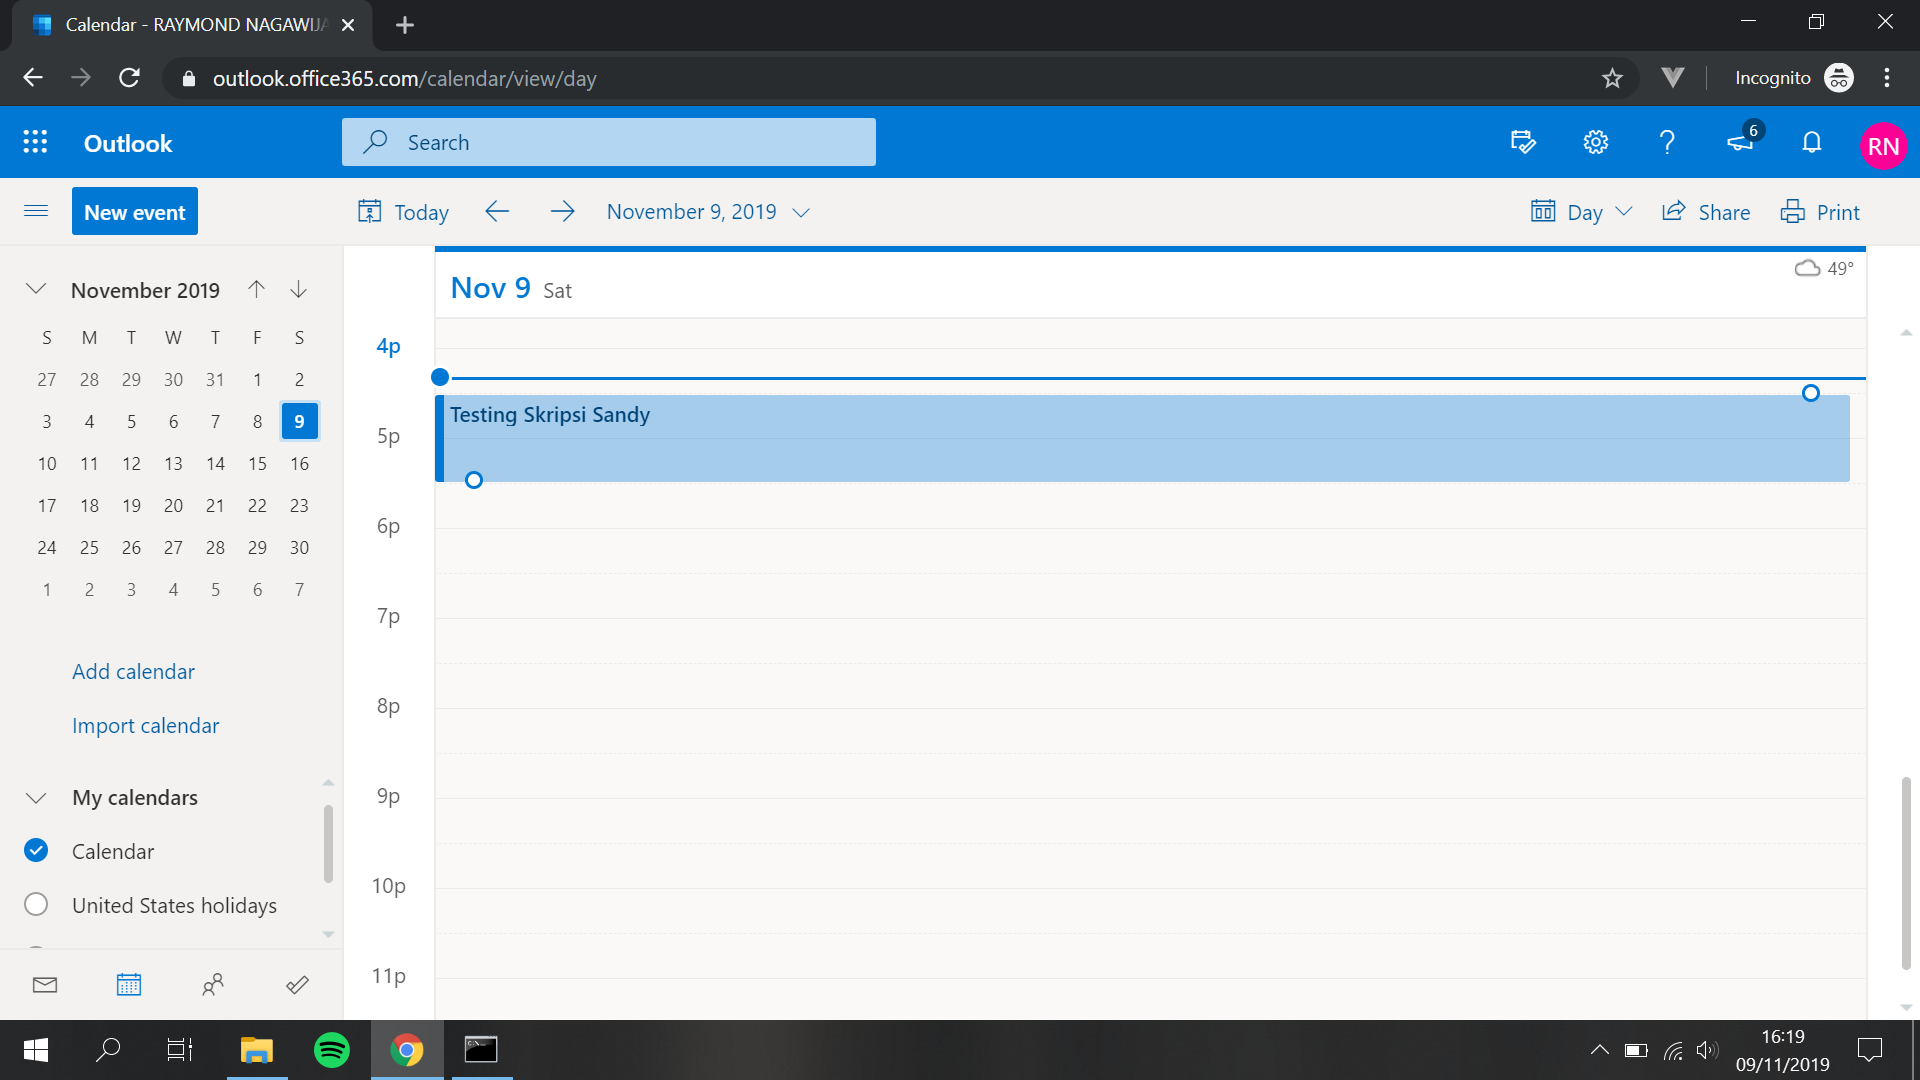
\includegraphics[width=10cm]{./Gambar/PengujianRaymond/Outlook.png}
  \centering
  \caption{Tampilan \textit{event} yang dibuat pengguna(Raymond).}
  \label{fig:outlook_raymond}
\end{figure}

\begin{figure}[h]
  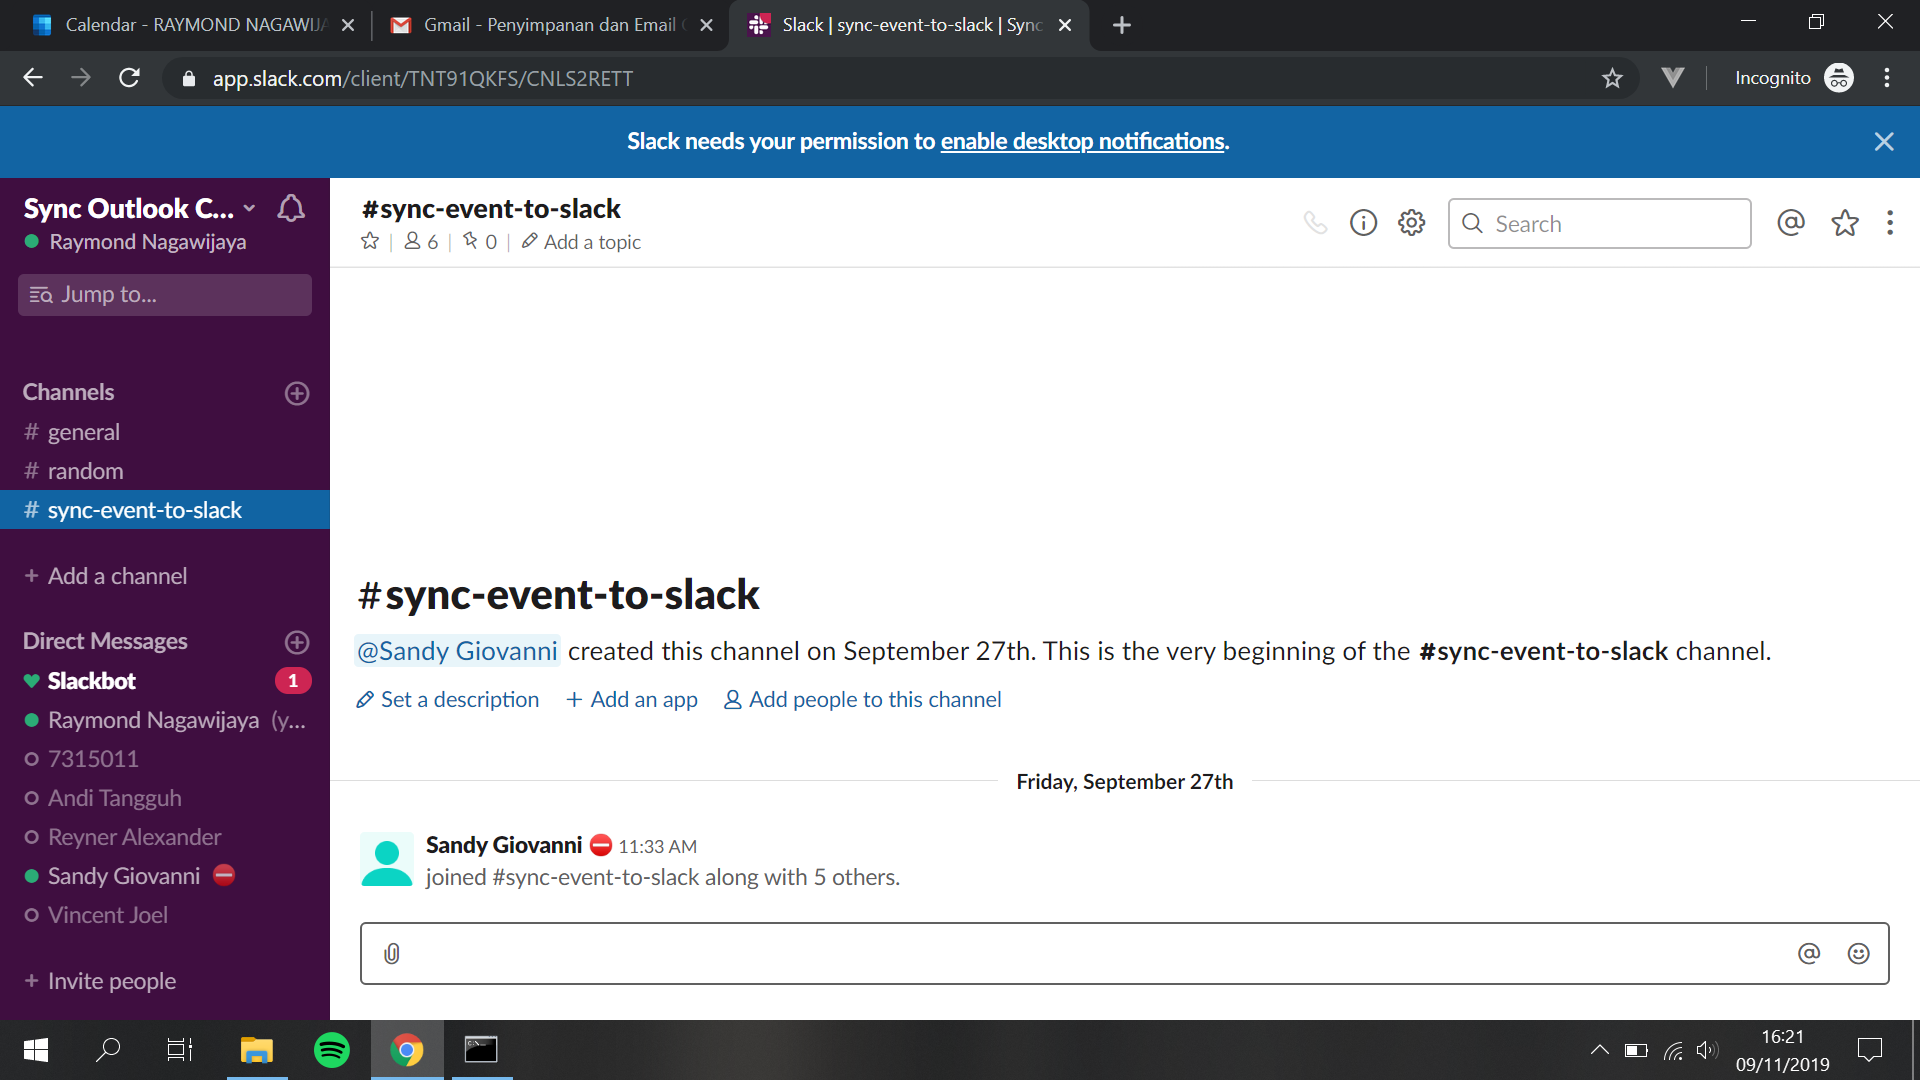
\includegraphics[width=10cm]{./Gambar/PengujianRaymond/Slack_Before.png}
  \centering
  \caption{Tampilan \textit{Slack} sebelum \textit{event} dimulai(Raymond).}
  \label{fig:slack_before_raymond}
\end{figure}

\begin{figure}[h]
  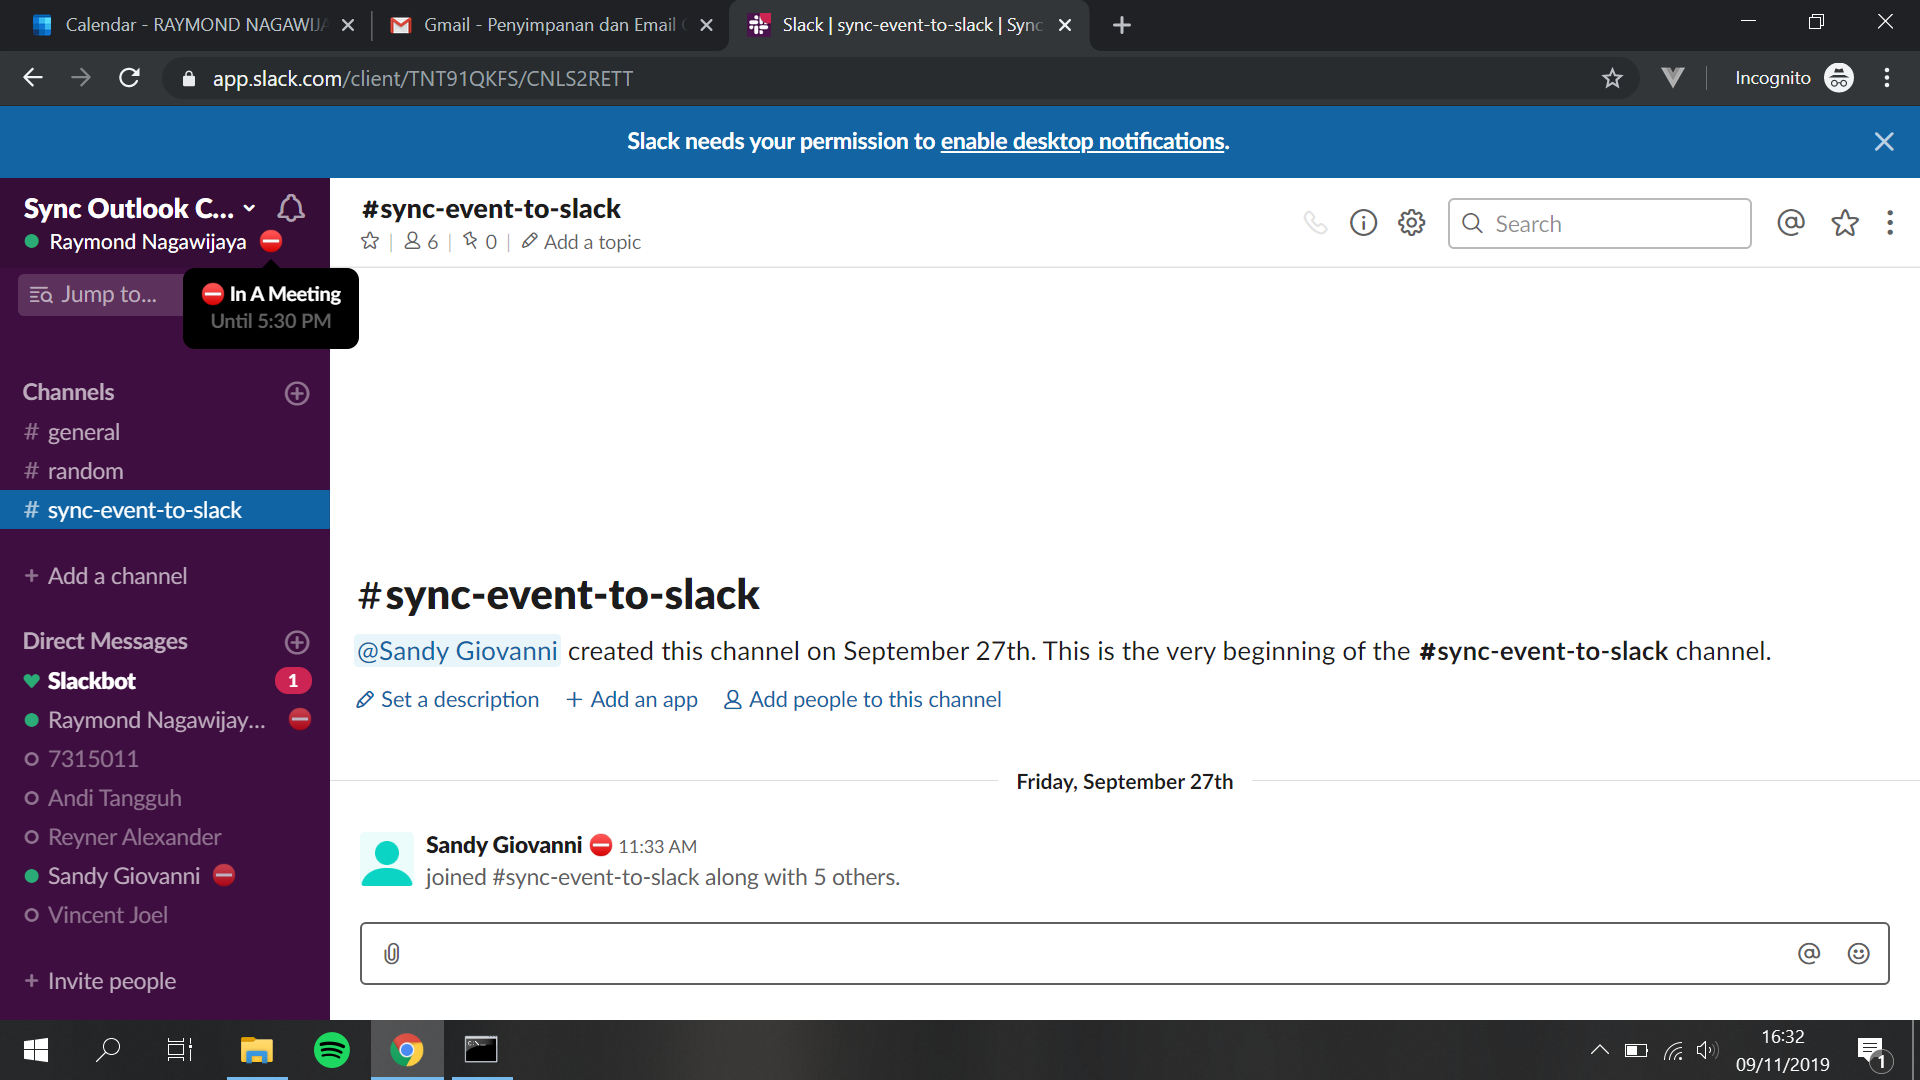
\includegraphics[width=10cm]{./Gambar/PengujianRaymond/Slack_After.png}
  \centering
  \caption{Tampilan \textit{Slack} setelah \textit{event} dimulai(Raymond).}
  \label{fig:slack_after_raymond}
\end{figure}

Dari gambar \ref{fig:outlook_raymond} sampai gambar \ref{fig:slack_after_raymond} merupakan bukti yang diambil dari pengguna yang melakukan pengujian yang bernama Raymond. Pada gambar \ref{fig:outlook_raymond} merupakan bukti bahwa Raymond sudah membuat sebuah \textit{event} pada waktu 16.30 dan gambar \ref{fig:slack_before_raymond} menunjukkan kondisi \textit{Slack} pada pukul 16.21 yang tidak memperlihatkan adanya status yang terpasang pada akun pengguna. Lalu pada gambar \ref{fig:slack_after_raymond} menunjukkan kondisi \textit{Slack} pada pukul 16.32 yang memperlihatkan adanya status yang terpasang pada akun pengguna yang status itu akan terpasang hingga waktu \textit{event} berakhir yaitu pukul 5.30. 
\clearpage

\begin{figure}[h]
  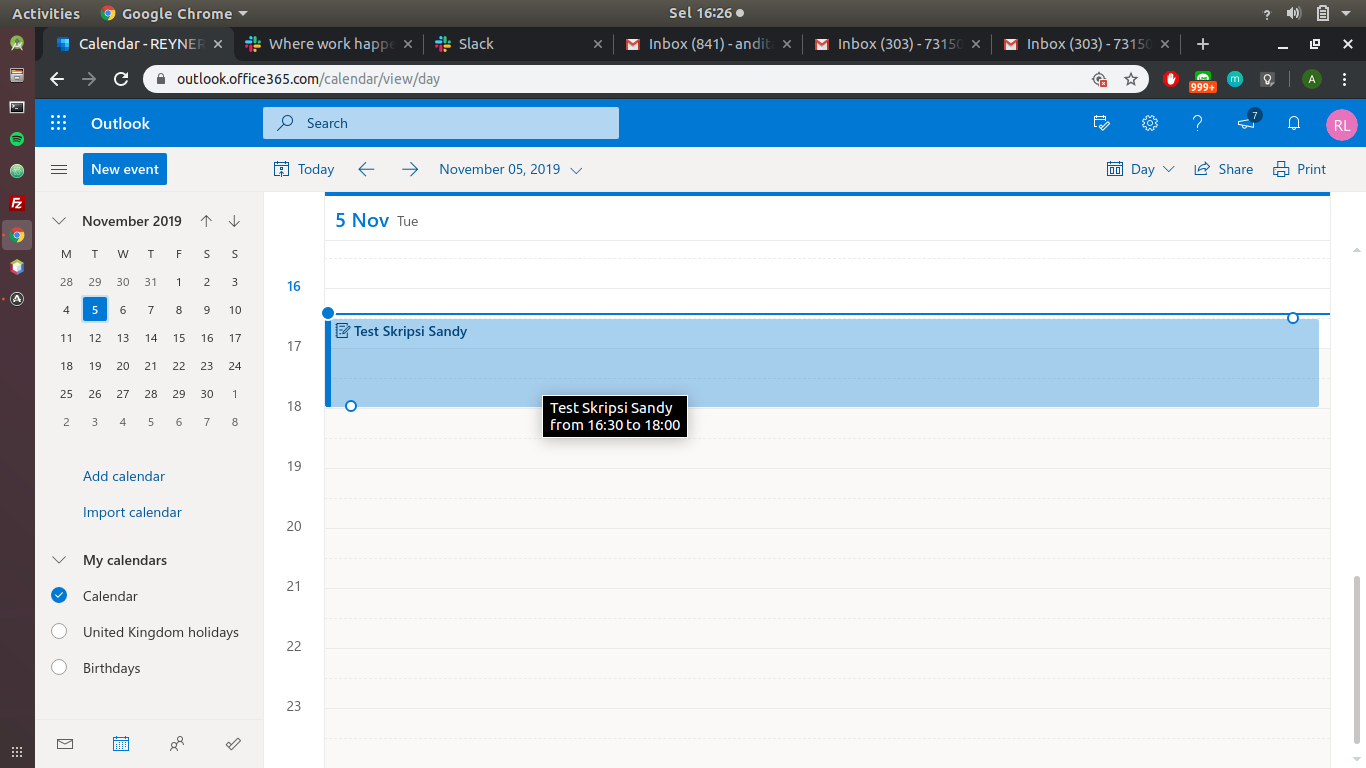
\includegraphics[width=10cm]{./Gambar/PengujianReyner/Outlook.png}
  \centering
  \caption{Tampilan \textit{event} yang dibuat pengguna(Reyner).}
  \label{fig:outlook_reyner}
\end{figure}

\begin{figure}[h]
  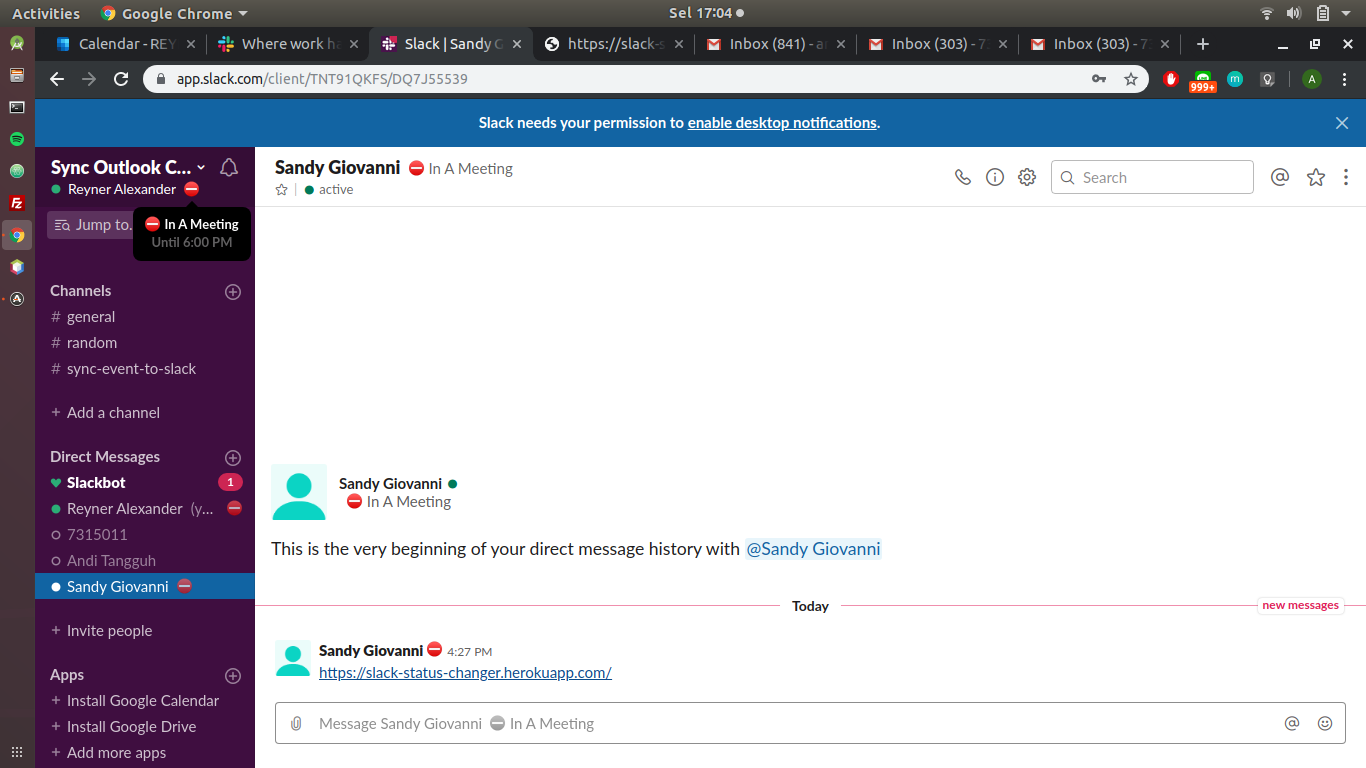
\includegraphics[width=10cm]{./Gambar/PengujianReyner/Slack_After.png}
  \centering
  \caption{Tampilan \textit{Slack} setelah \textit{event} dimulai(Reyner).}
  \label{fig:slack_after_reyner}
\end{figure}

Dari gambar \ref{fig:outlook_reyner} sampai gambar \ref{fig:slack_after_reyner} merupakan bukti dari hasil pengujian dari pengguna yang bernama Reyner. Pada gambar \ref{fig:outlook_reyner} dapat dilihat bahwa pengguna memiliki sebuah \textit{event} yang dimulai pada pukul 16.30 dan berakhir pada pukul 18.00. Lalu pada gambar \ref{fig:slack_after_reyner} dapat dilihat bahwa status pengguna telah berubah dan status itu berlaku sampai pukul 18.00 tepat saat \textit{event} berakhir. 
\clearpage

\begin{figure}[h]
  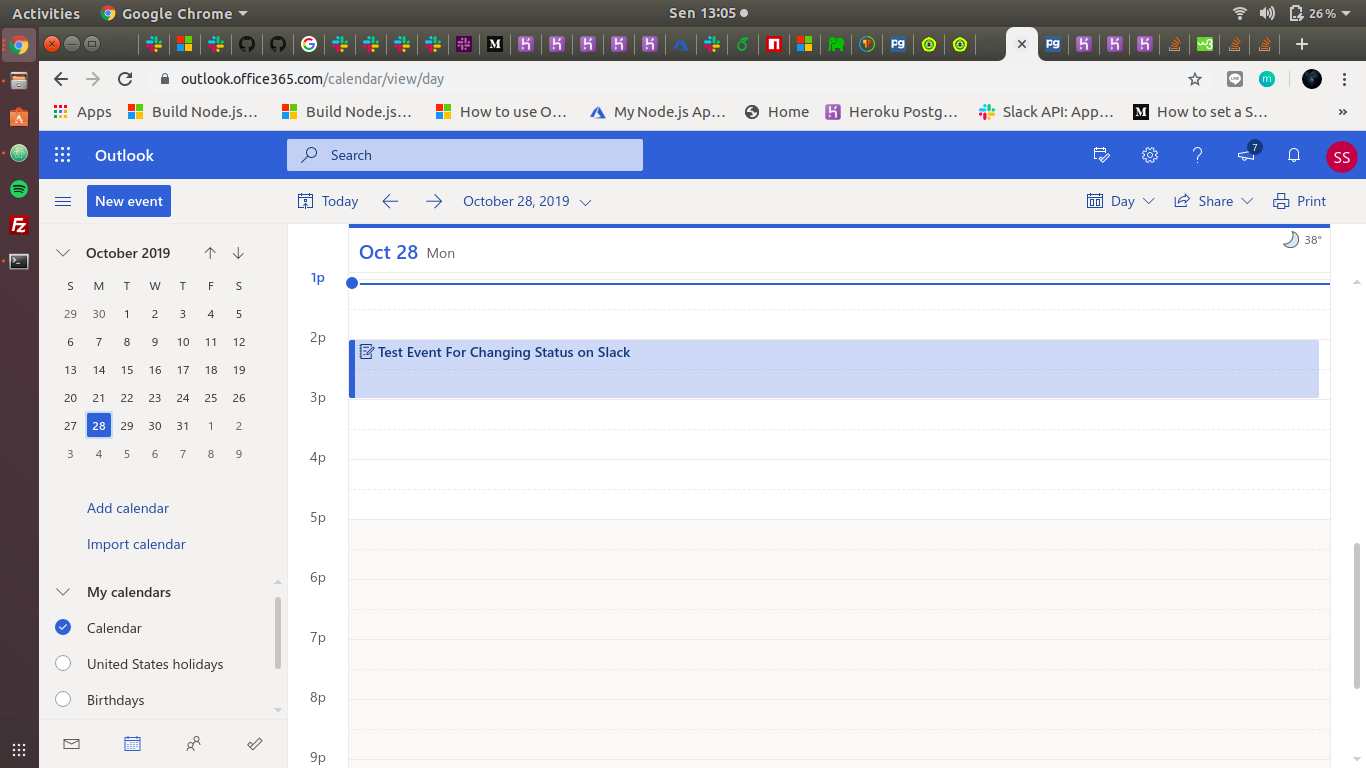
\includegraphics[width=10cm]{./Gambar/PengujianSandy/Outlook.png}
  \centering
  \caption{Tampilan \textit{event} yang dibuat pengguna(Sandy).}
  \label{fig:outlook_sandy}
\end{figure}

\begin{figure}[h]
  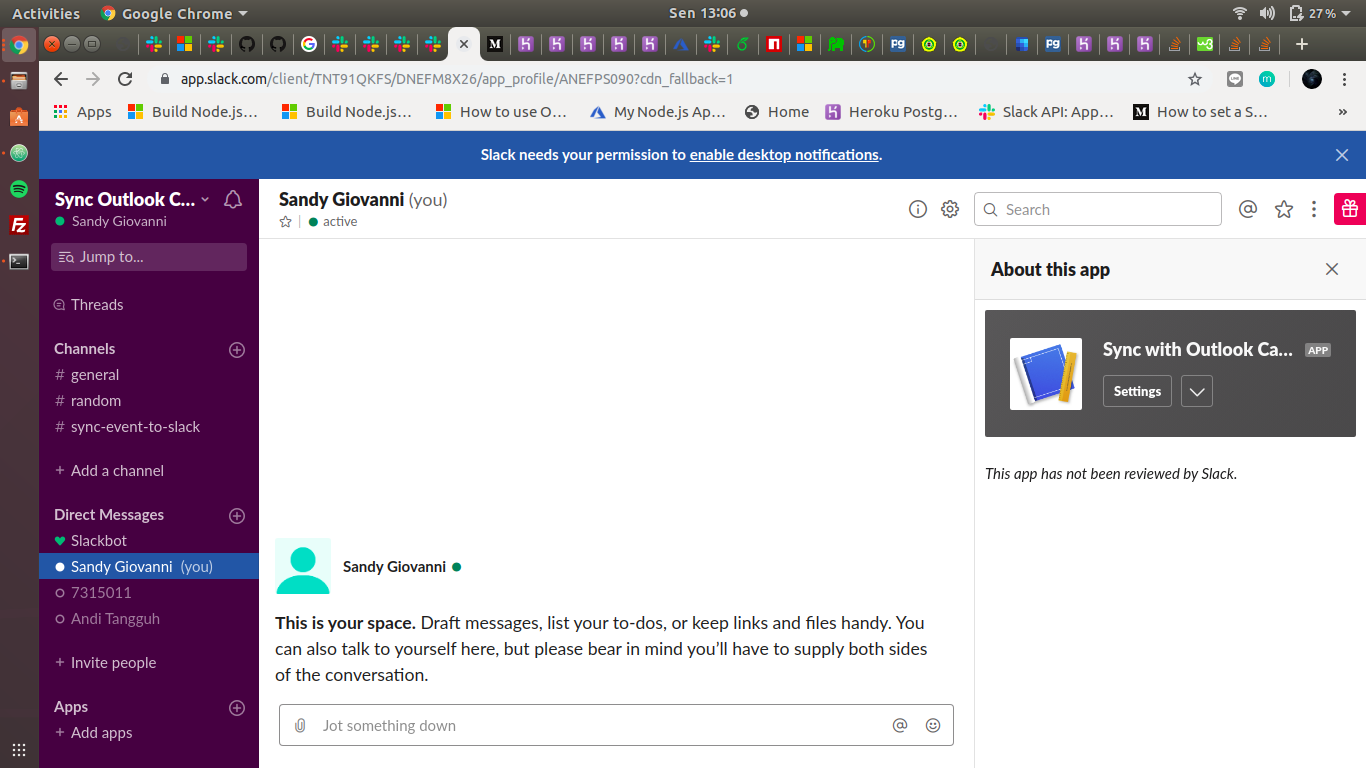
\includegraphics[width=10cm]{./Gambar/PengujianSandy/Slack_Before.png}
  \centering
  \caption{Tampilan \textit{Slack} sebelum \textit{event} dimulai(Sandy).}
  \label{fig:slack_before_sandy}
\end{figure}

\begin{figure}[h]
  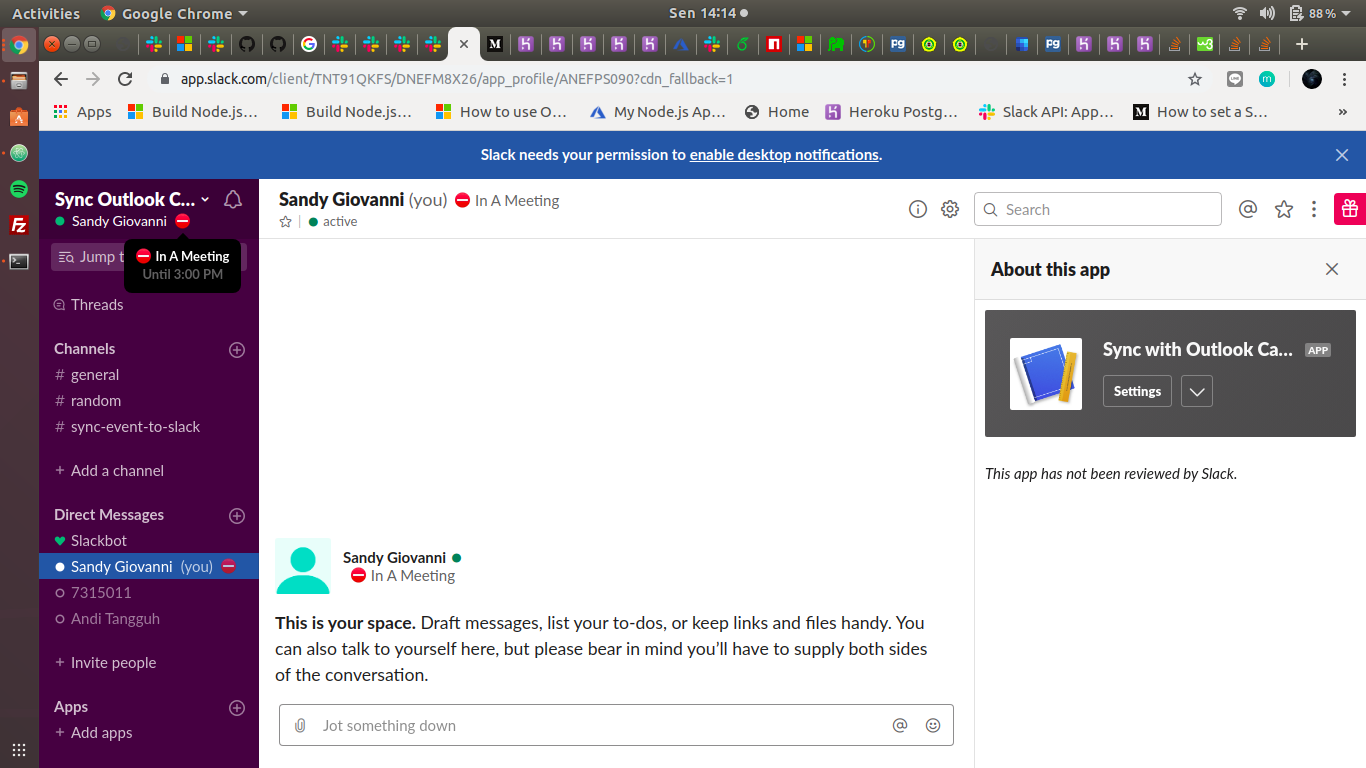
\includegraphics[width=10cm]{./Gambar/PengujianSandy/Slack_After.png}
  \centering
  \caption{Tampilan \textit{Slack} setelah \textit{event} dimulai(Sandy).}
  \label{fig:slack_after_sandy}
\end{figure}

Pada gambar \ref{fig:outlook_sandy} sampai gambar \ref{fig:slack_after_sandy} merupakan bukti hasil pengujian yang dilakukan oleh pengguna bernama Sandy. Pada gambar \ref{fig:outlook_sandy} terlihat bahwa ada \textit{event} yang tercatat akan dimulai pada pukul 14.00 dan pada pukul 13.06 belum ada status yang tertulis di akun pengguna yang terekam dalam gambar \ref{fig:slack_before_sandy}. Lalu pada pukul 14.14 status muncul dalam akun pengguna yang status itu akan hilang pada pukul 15.00 sesuai dengan yang tertulis di dalam \textit{Outlook Calendar}. 
\clearpage

\begin{figure}[h]
  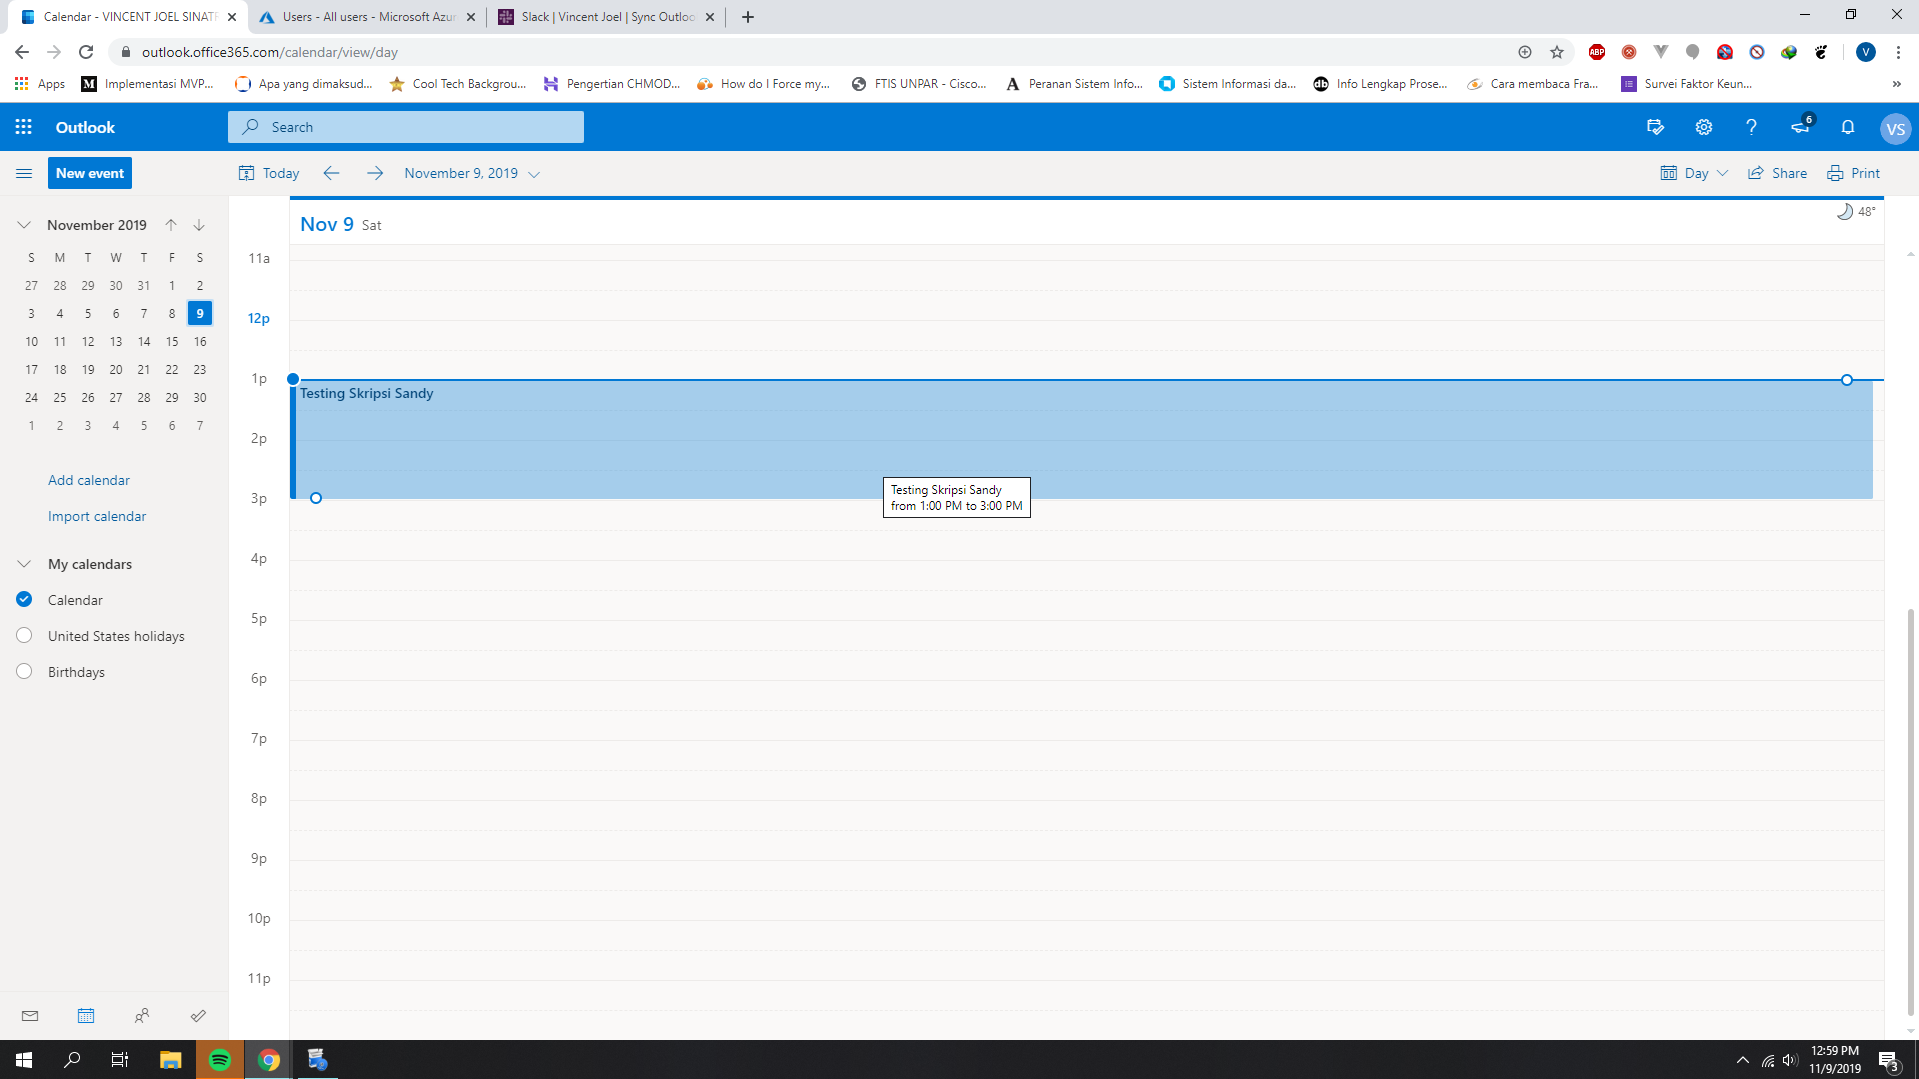
\includegraphics[width=10cm]{./Gambar/PengujianVincent/Outlook.png}
  \centering
  \caption{Tampilan \textit{event} yang dibuat pengguna(Vincent).}
  \label{fig:outlook_vincent}
\end{figure}

\begin{figure}[h]
  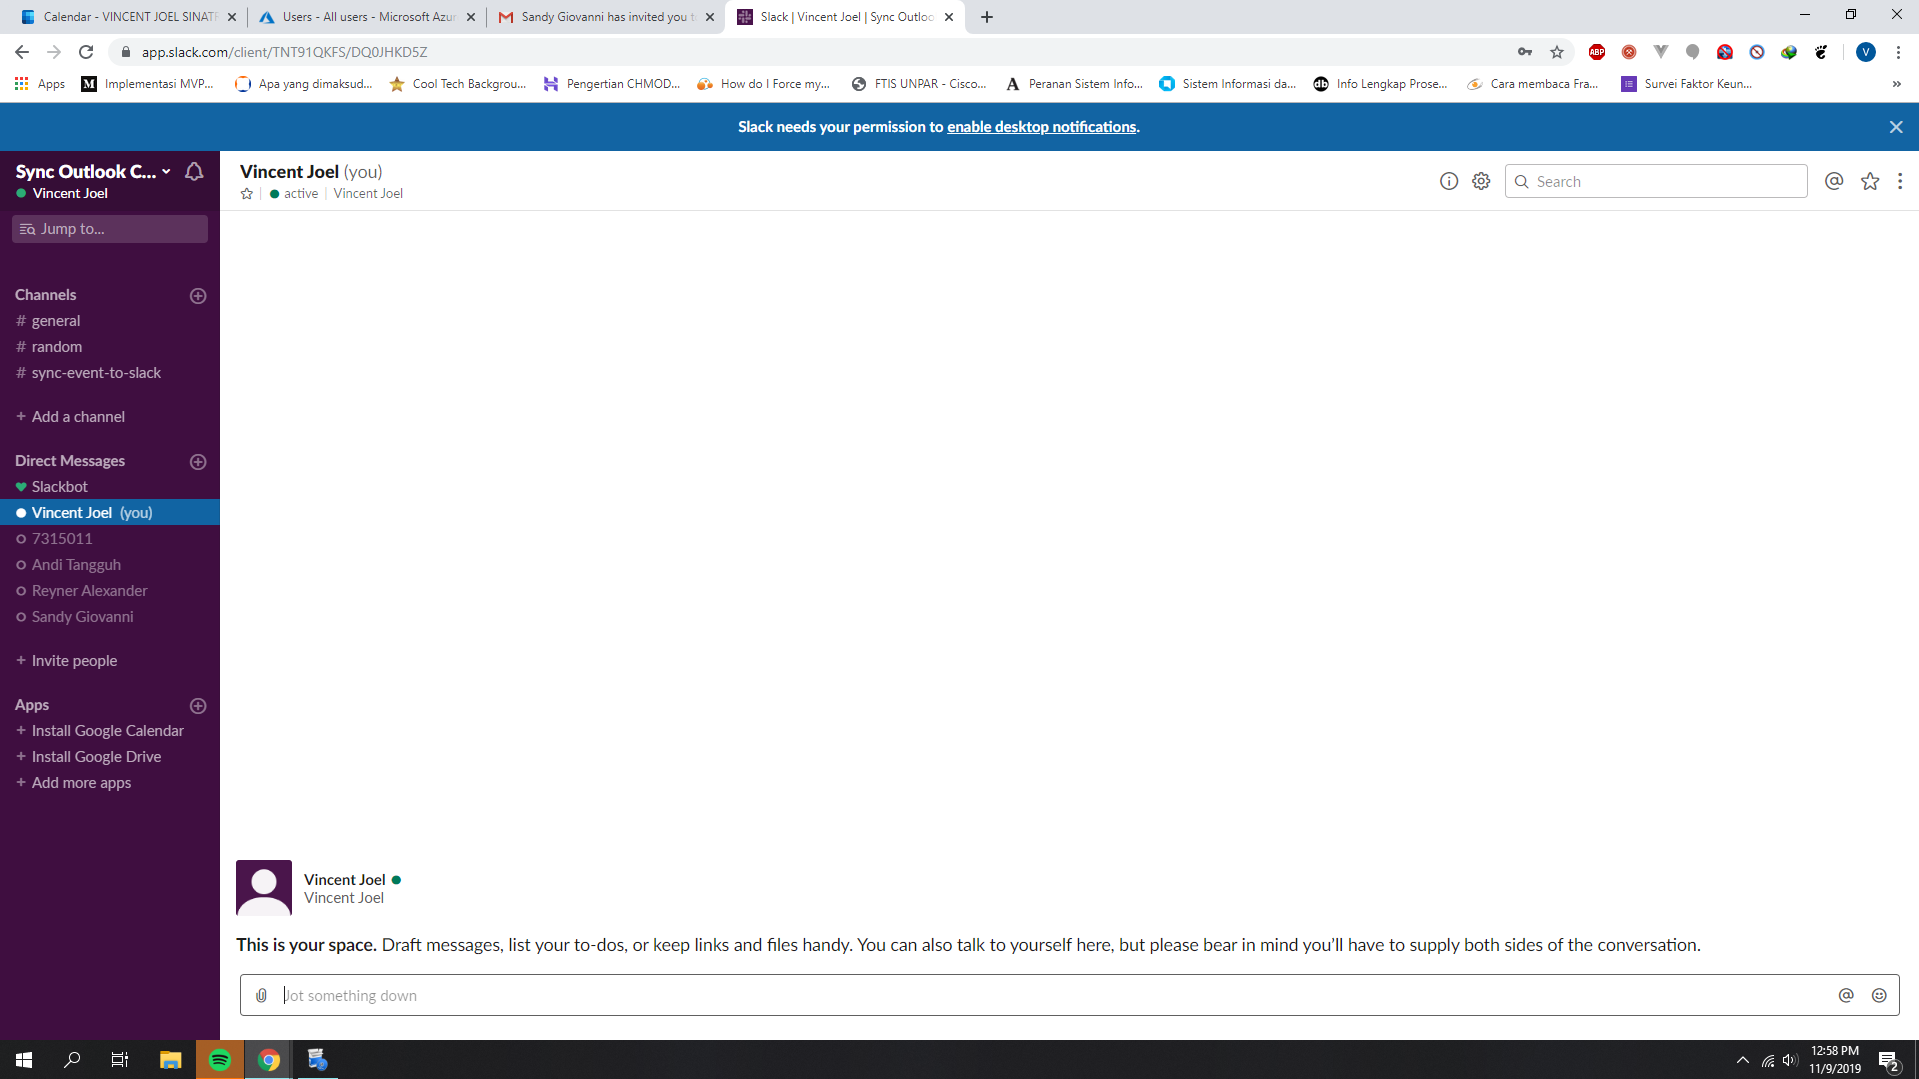
\includegraphics[width=10cm]{./Gambar/PengujianVincent/Slack_Before.png}
  \centering
  \caption{Tampilan \textit{Slack} sebelum \textit{event} dimulai(Vincent).}
  \label{fig:slack_before_vincent}
\end{figure}

\begin{figure}[h]
  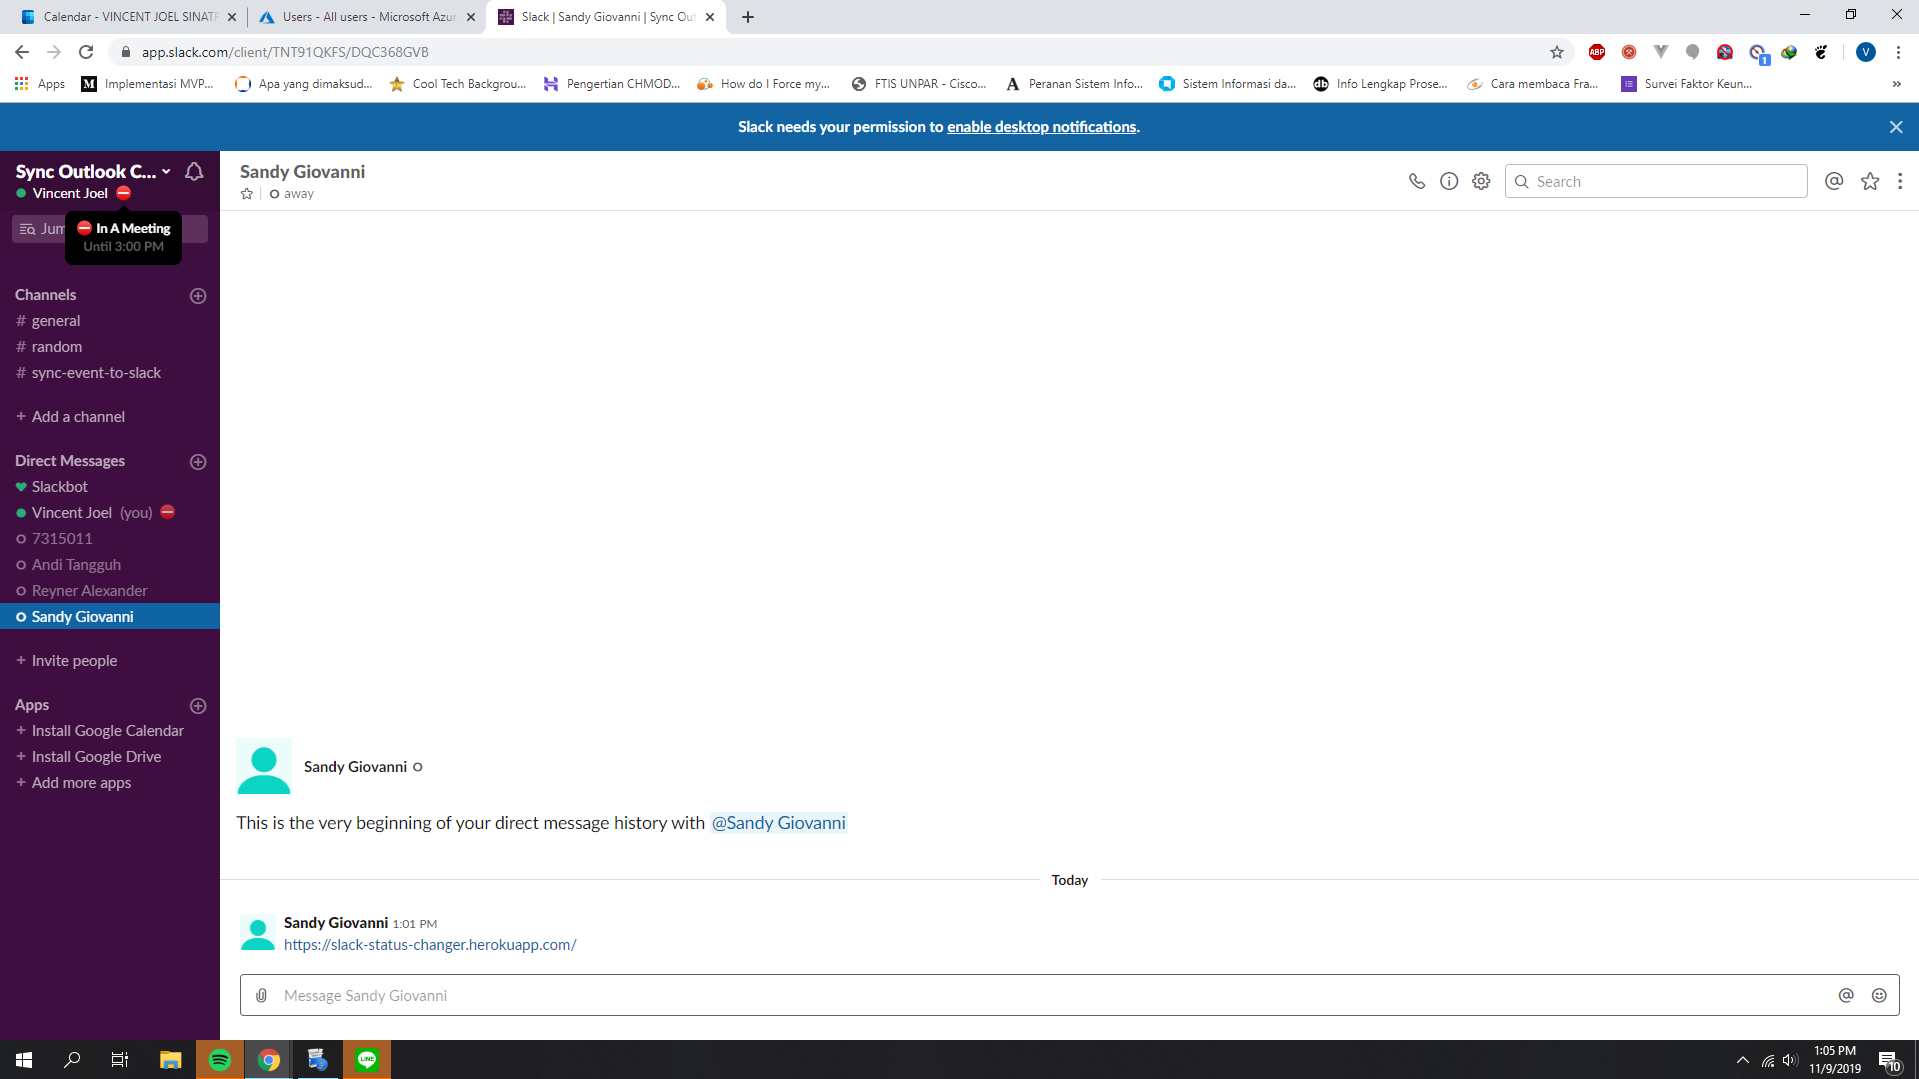
\includegraphics[width=10cm]{./Gambar/PengujianVincent/Slack_After.png}
  \centering
  \caption{Tampilan \textit{Slack} setelah \textit{event} dimulai(Vincent).}
  \label{fig:slack_after_vincent}
\end{figure}

Pada gambar \ref{fig:outlook_vincent} sampai dengan gambar \ref{fig:slack_after_vincent} merupakan hasil dari pengujian yang dilakukan pengguna bernama Vincent. Pada gambar \ref{fig:outlook_vincent} terlihat ada sebuah \textit{event} yang akan dimulai pada pukul 13.00 dan pada gambar \ref{fig:slack_before_vincent} dapat terlihat bahwa pada pukul 12.58 tidak ada status di dalam akun pengguna lalu pada pukul 13.05 terdapat status dalam akun pengguna yang statusnya akan hilang pada pukul 15.00 seperti di gambar \ref{fig:slack_after_vincent} sesuai dengan keterangan \textit{event} yang terdapat pada \textit{Outlook Calendar}. 
\clearpage

\begin{figure}[h]
  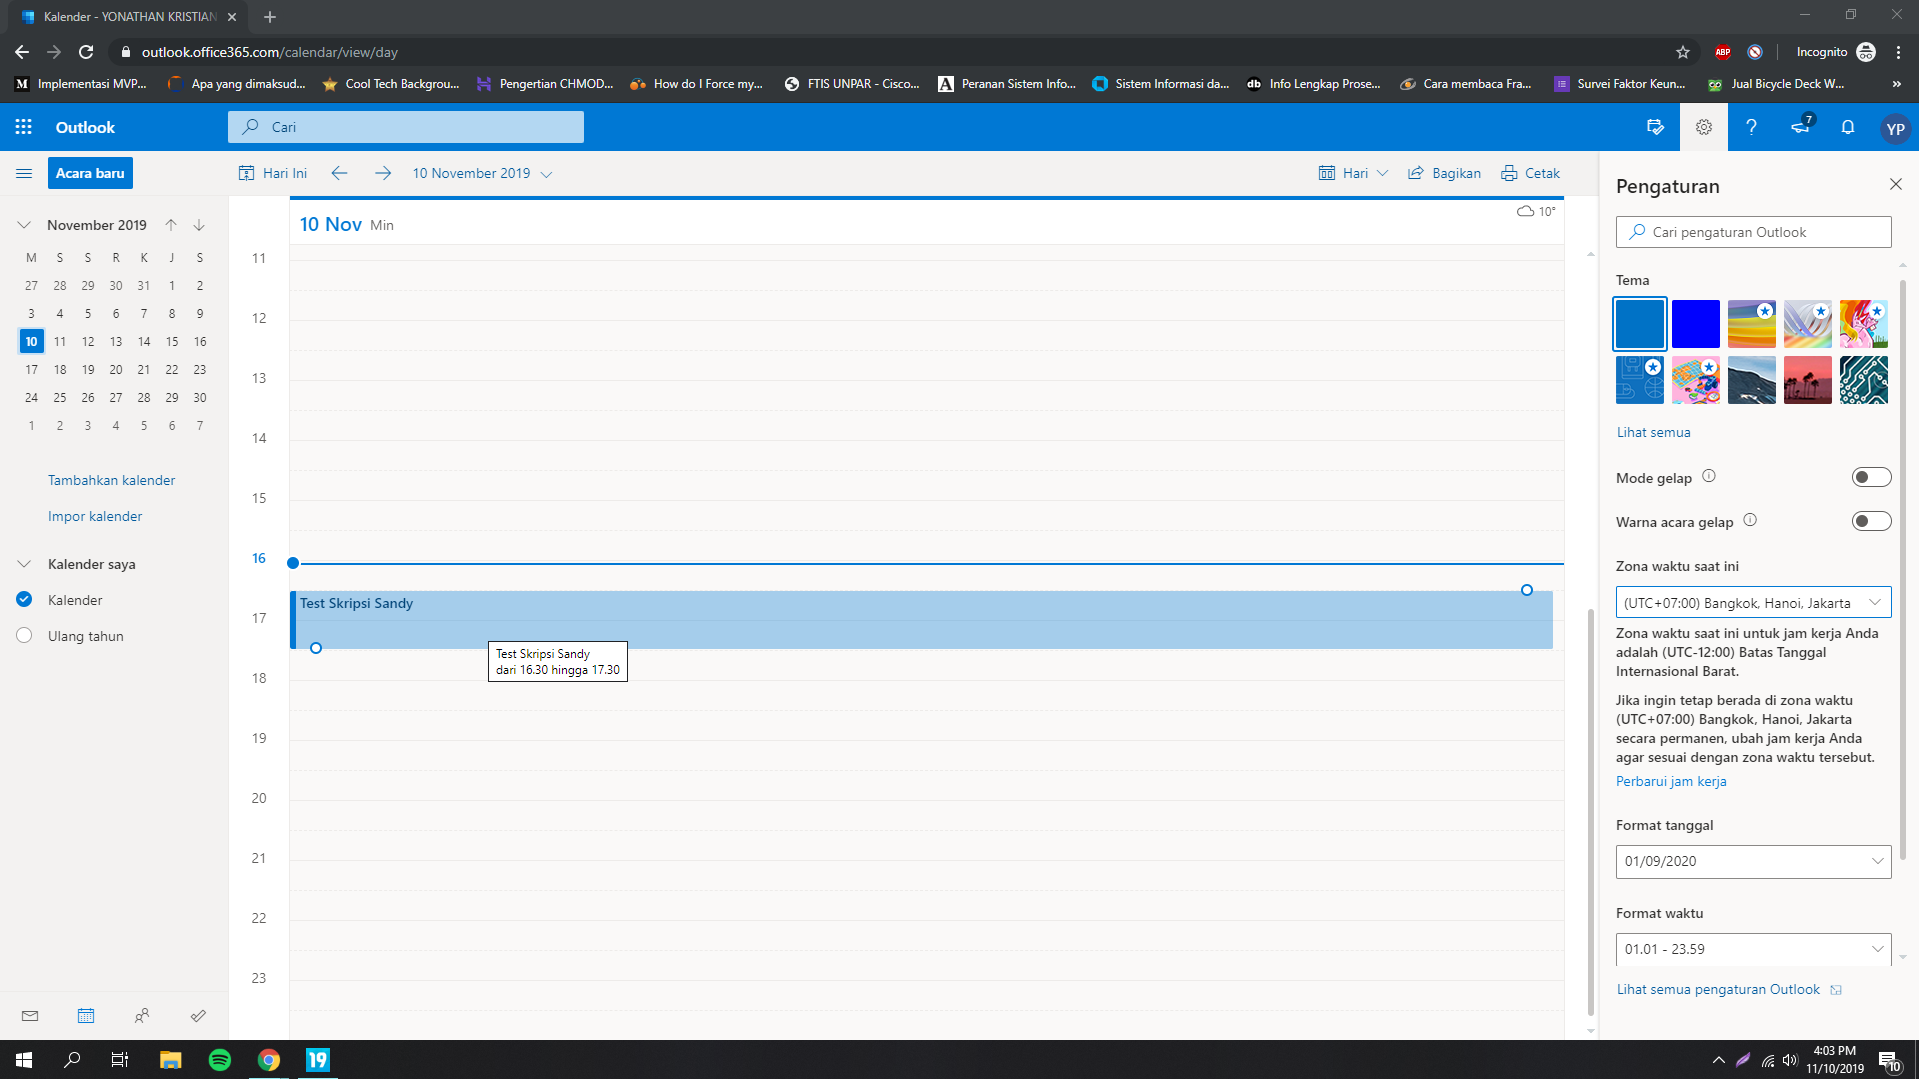
\includegraphics[width=10cm]{./Gambar/PengujianYonathan/Outlook.png}
  \centering
  \caption{Tampilan \textit{event} yang dibuat pengguna(Yonathan).}
  \label{fig:outlook_yonathan}
\end{figure}

\begin{figure}[h]
  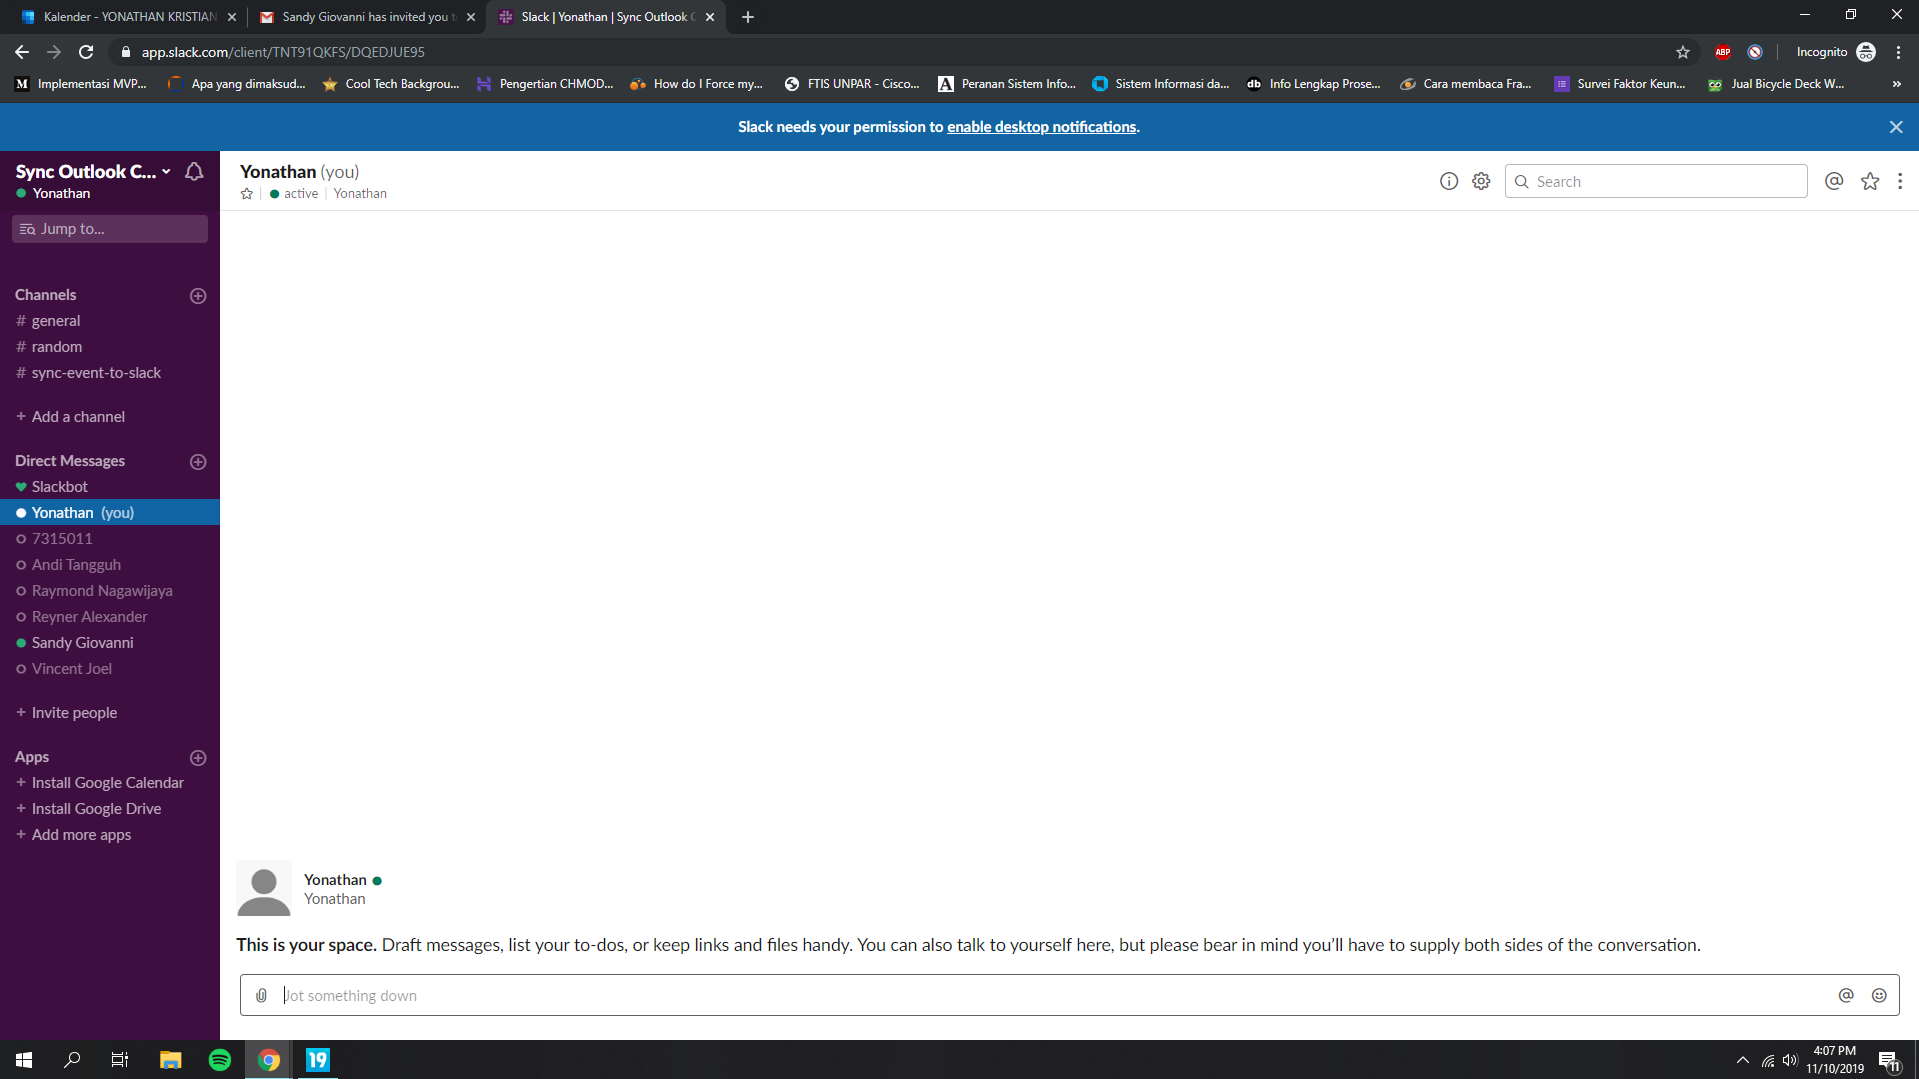
\includegraphics[width=10cm]{./Gambar/PengujianYonathan/Slack_Before.png}
  \centering
  \caption{Tampilan \textit{Slack} sebelum \textit{event} dimulai(Yonathan).}
  \label{fig:slack_before_yonathan}
\end{figure}

\begin{figure}[h]
  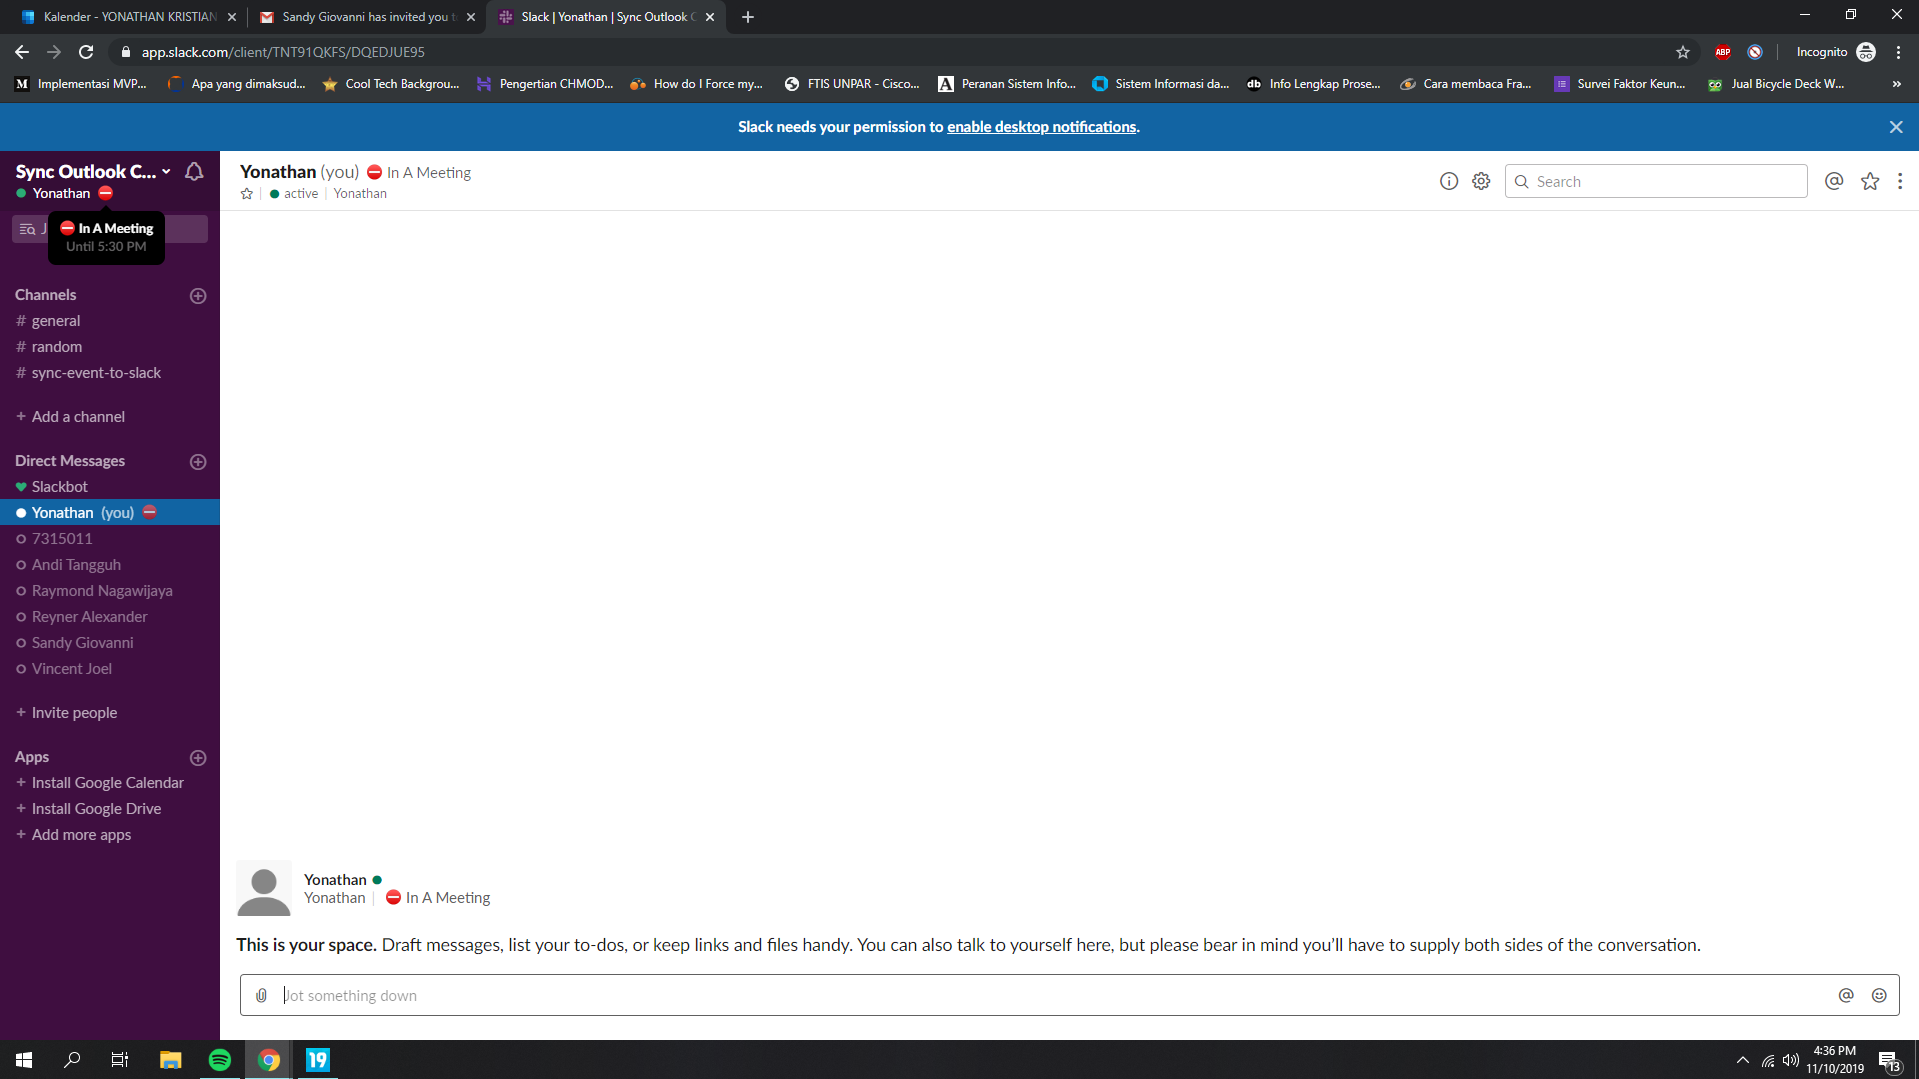
\includegraphics[width=10cm]{./Gambar/PengujianYonathan/Slack_After.png}
  \centering
  \caption{Tampilan \textit{Slack} setelah \textit{event} dimulai(Yonathan).}
  \label{fig:slack_after_yonathan}
\end{figure}

Pada gambar \ref{fig:outlook_yonathan} sampai dengan gambar \ref{fig:slack_after_yonathan} merupakan hasil dari pengujian yang dilakukan oleh pengguna bernama Yonathan. Di gambar \ref{fig:outlook_yonathan} terdapat \textit{event} yang mulai pada pukul 16.30 dan pada gambar \ref{fig:slack_before_yonathan} yang diambil pada pukul 16.07, belum ada status yang terpasang di akun pengguna. Pada gambar \ref{fig:slack_after_yonathan} yang diambil pada pukul 16.36 sudah ada status yang terpasang di akun pengguna dan status itu akan hilang pada pukul 17.30 yang sesuai dengan \textit{event} yang tercatat pada \textit{Outlook Calendar}. 
\clearpage

\subsection{Pengujian Eksperimental}
\subsubsection{Skenario Pengujian}
Pengujian eksperimental ini dilakukan dengan pengguna-pengguna yang tergabung dalam \textit{workspace} di luar dari \textit{workspace} tempat perangkat lunak ini didaftarkan. Pengguna harus memiliki \textit{Outlook Calendar} dan juga pengguna membuat sebuah \textit{event} yang didaftarkan di dalam \textit{Outlook Calendar}.
\subsubsection{Tujuan Pengujian}
Tujuan dari pengujian ini adalah untuk mengetahui bahwa perangkat lunak yang didaftarkan di satu \textit{workspace} di dalam \textit{Slack} tidak hanya terikat pada satu \textit{workspace} itu saja tetapi bisa digunakan ke \textit{workspace} lainnya asalkan pengaturan saat pendaftaran perangkat lunak di dalam \textit{Slack} mengaktifkan ``\textit{Manage Distribution}''. 
\subsubsection{Hasil Pengujian}
Dari gambar \ref{fig:outlook_chris} sampai dengan gambar \ref{fig:slack_after_yosua} merupakan hasil dari para pengguna yang bersedia untuk menguji perangkat lunak di \textit{workspace} yang dimiliki masing-masing atau di luar dari \textit{workspace} tempat perangkat lunak ini didaftarkan. 

\begin{figure}[h]
  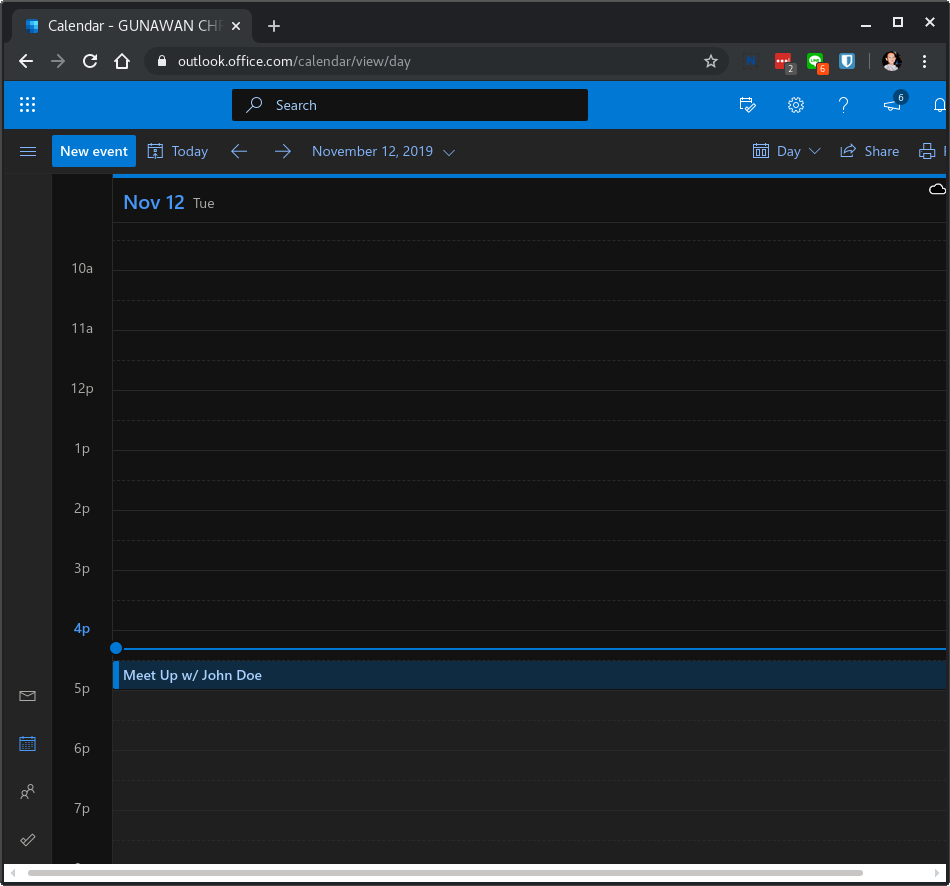
\includegraphics[width=10cm]{./Gambar/PengujianChris/Outlook.png}
  \centering
  \caption{Tampilan \textit{event} yang dibuat pengguna(Chris).}
  \label{fig:outlook_chris}
\end{figure}

\begin{figure}[h]
  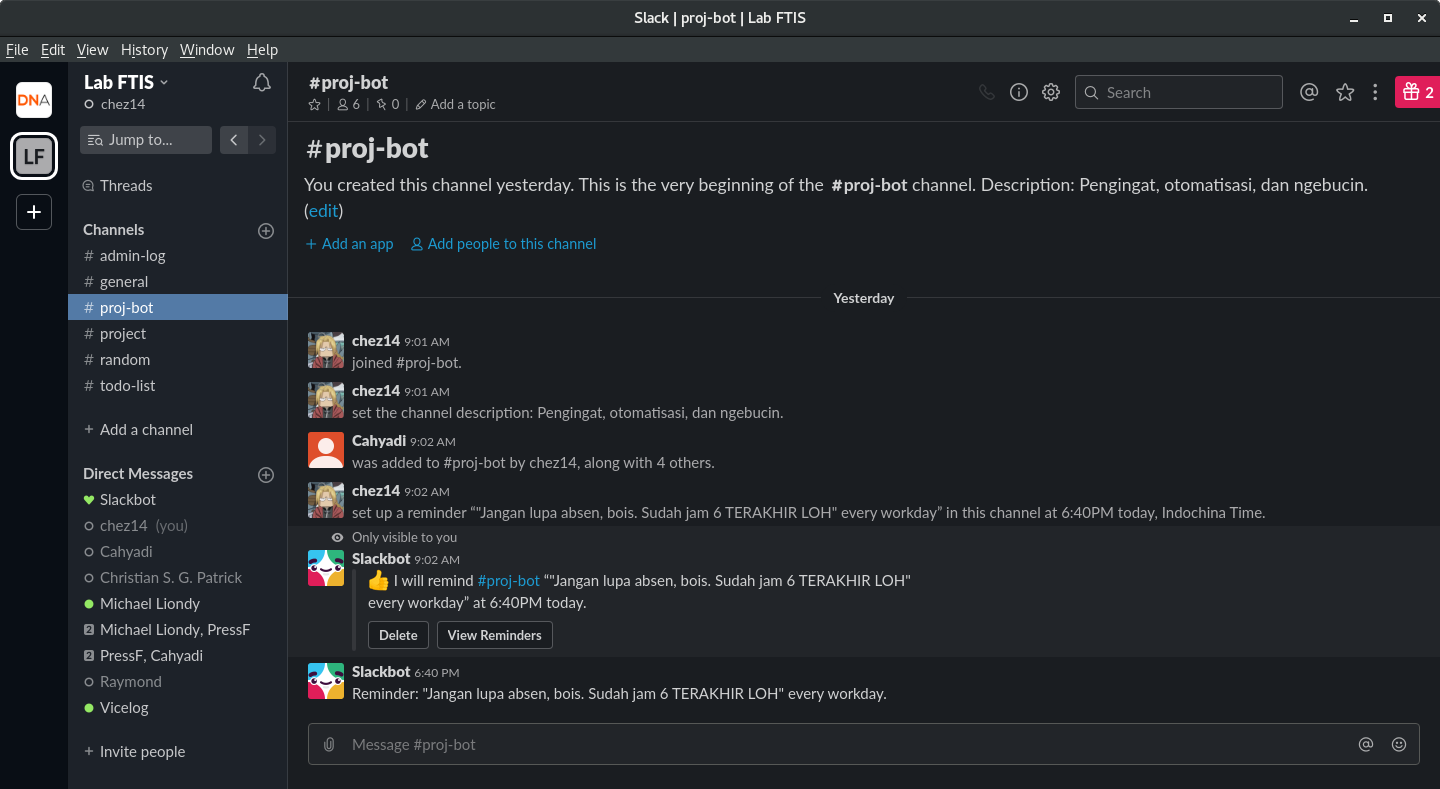
\includegraphics[width=10cm]{./Gambar/PengujianChris/Slack_Before.png}
  \centering
  \caption{Tampilan \textit{Slack} sebelum \textit{event} dimulai(Chris).}
  \label{fig:slack_before_chris}
\end{figure}

\begin{figure}[h]
  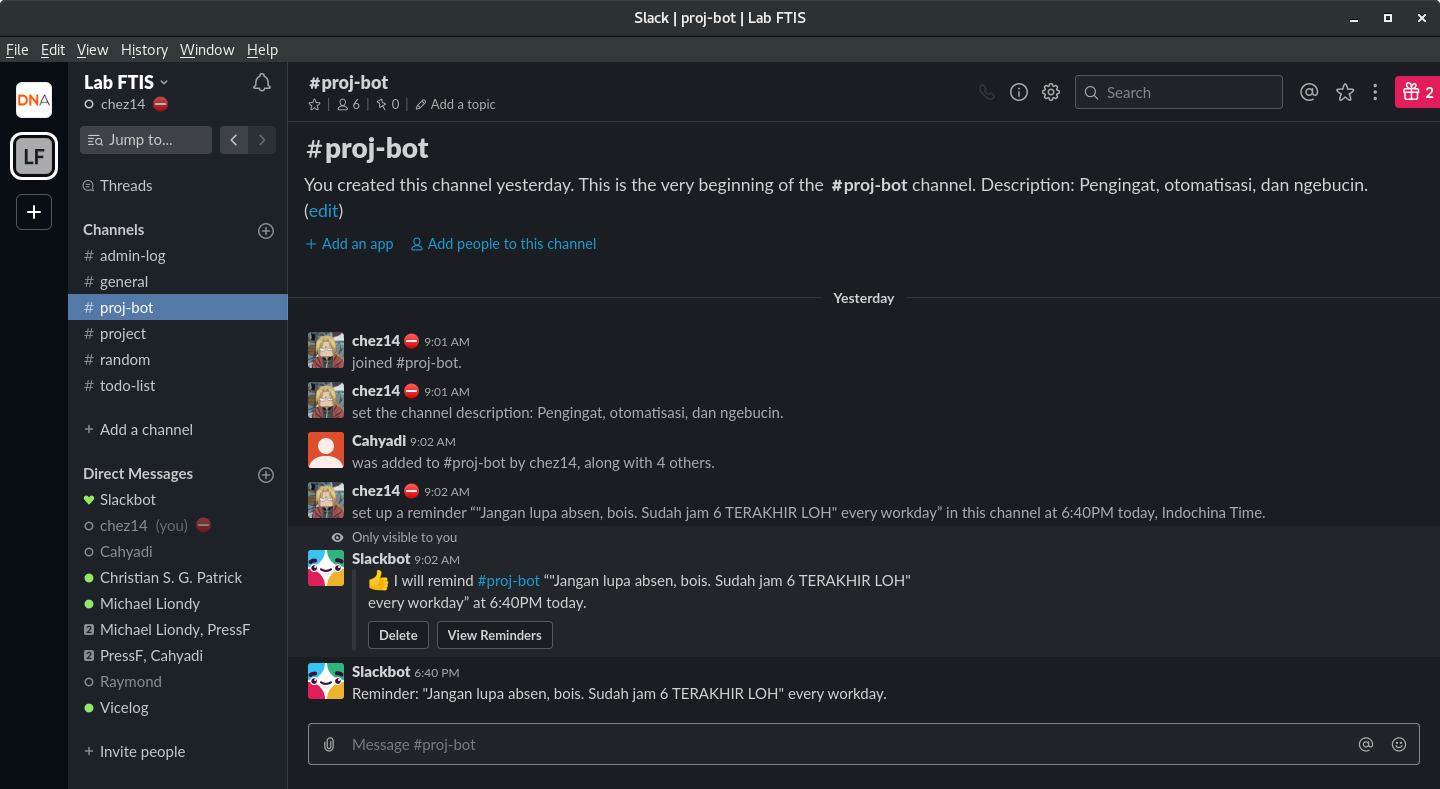
\includegraphics[width=10cm]{./Gambar/PengujianChris/Slack_After.png}
  \centering
  \caption{Tampilan \textit{Slack} setelah \textit{event} dimulai(Chris).}
  \label{fig:slack_after_chris}
\end{figure}

Gambar \ref{fig:outlook_chris} sampai dengan gambar \ref{fig:slack_after_chris} merupakan hasil yang didapat dari pengguna yang bernama Chris yang merupakan seorang admin di lab FTIS. Pada gambar \ref{fig:outlook_chris} terlihat ada \textit{event} yang terdaftar pukul 16.30. Lalu pada gambar \ref{fig:slack_before_chris} belum terdapat status yang terpasang pada akun pengguna dan \textit{workspace} yang pengguna pakai adalah \textit{workspace} yang bernama Lab FTIS. Pada gambar \ref{fig:slack_after_chris} dapat terlihat bahwa status sudah terpasang pada akun pengguna. 
\clearpage

\begin{figure}[h]
  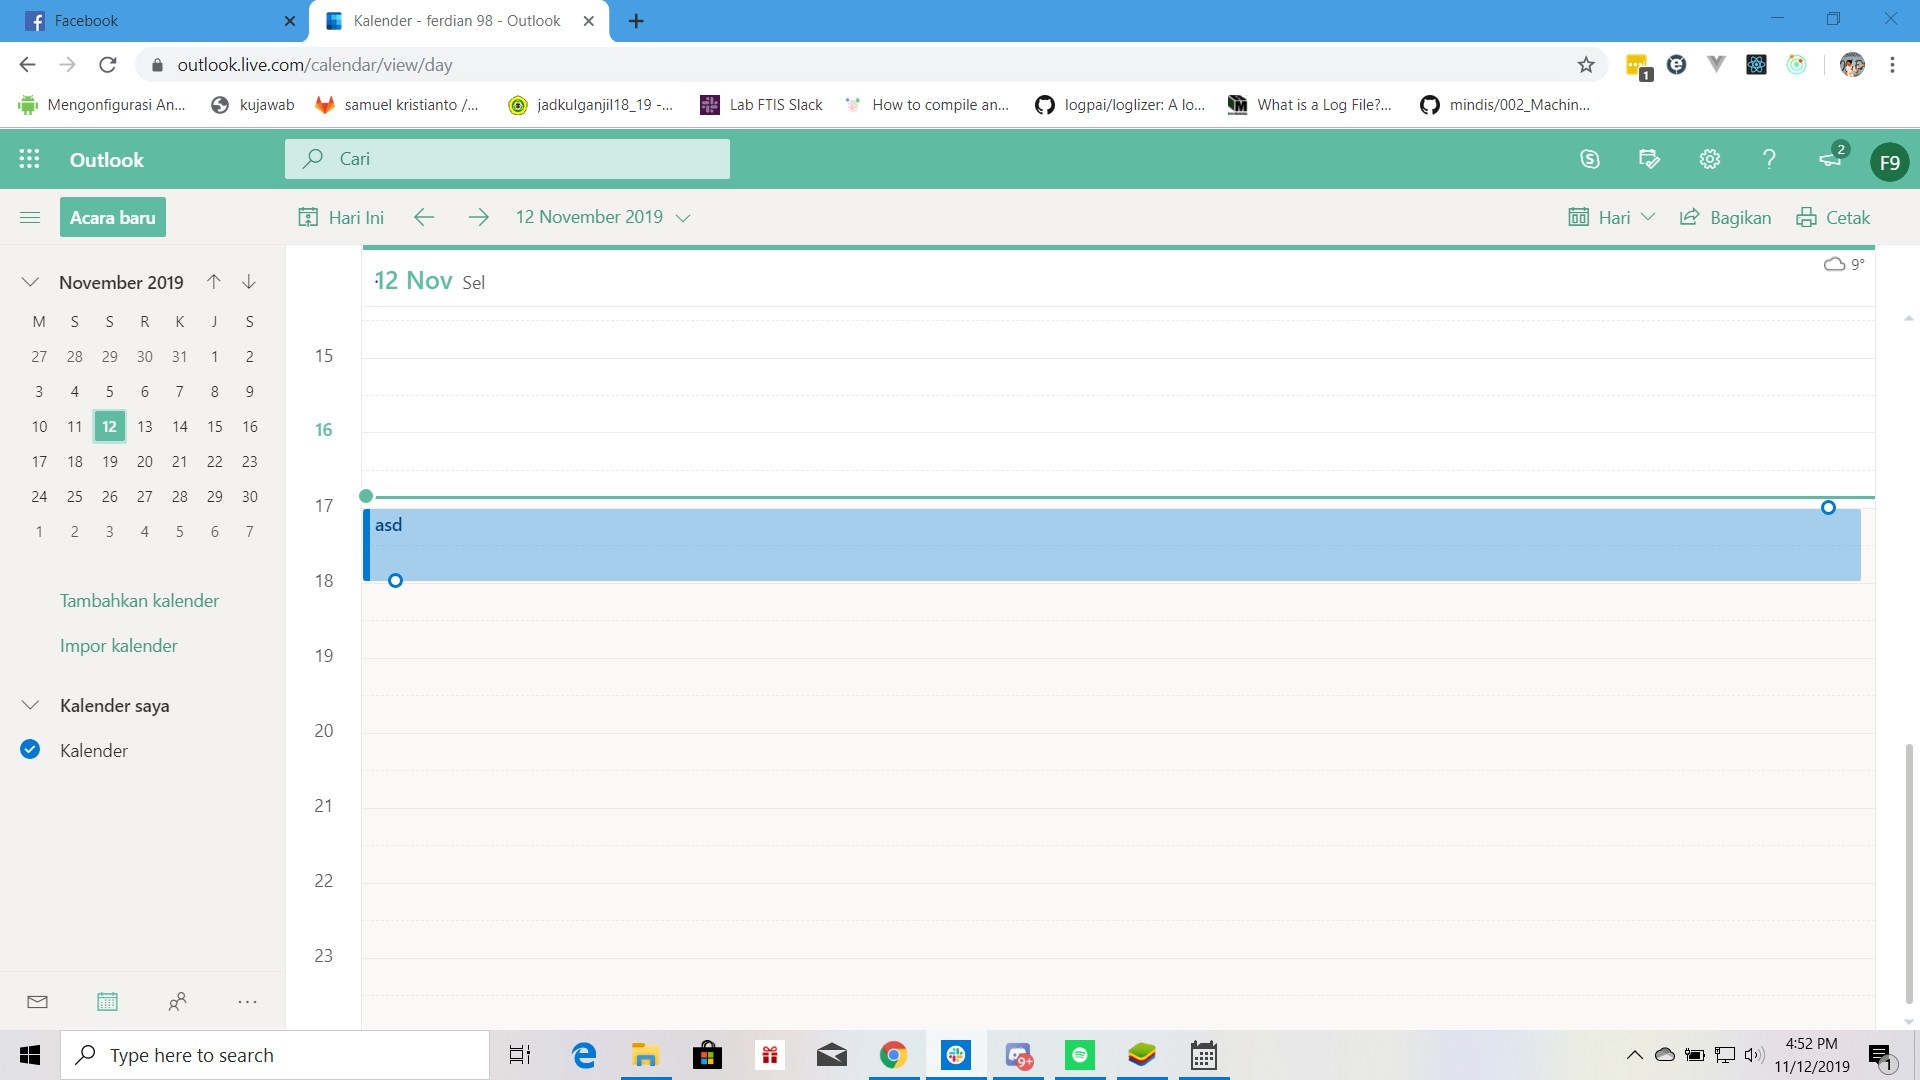
\includegraphics[width=10cm]{./Gambar/PengujianFerdian/Outlook.jpg}
  \centering
  \caption{Tampilan \textit{event} yang dibuat pengguna(Ferdian).}
  \label{fig:outlook_ferdian}
\end{figure}

\begin{figure}[h]
  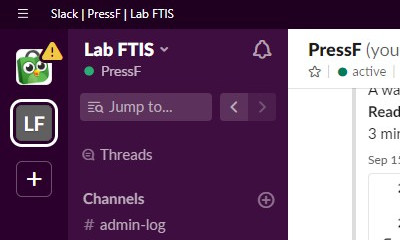
\includegraphics[width=10cm]{./Gambar/PengujianFerdian/Slack_Before(2).jpg}
  \centering
  \caption{Tampilan \textit{Slack} sebelum \textit{event} dimulai(Ferdian).}
  \label{fig:slack_before_ferdian}
\end{figure}

\begin{figure}[h]
  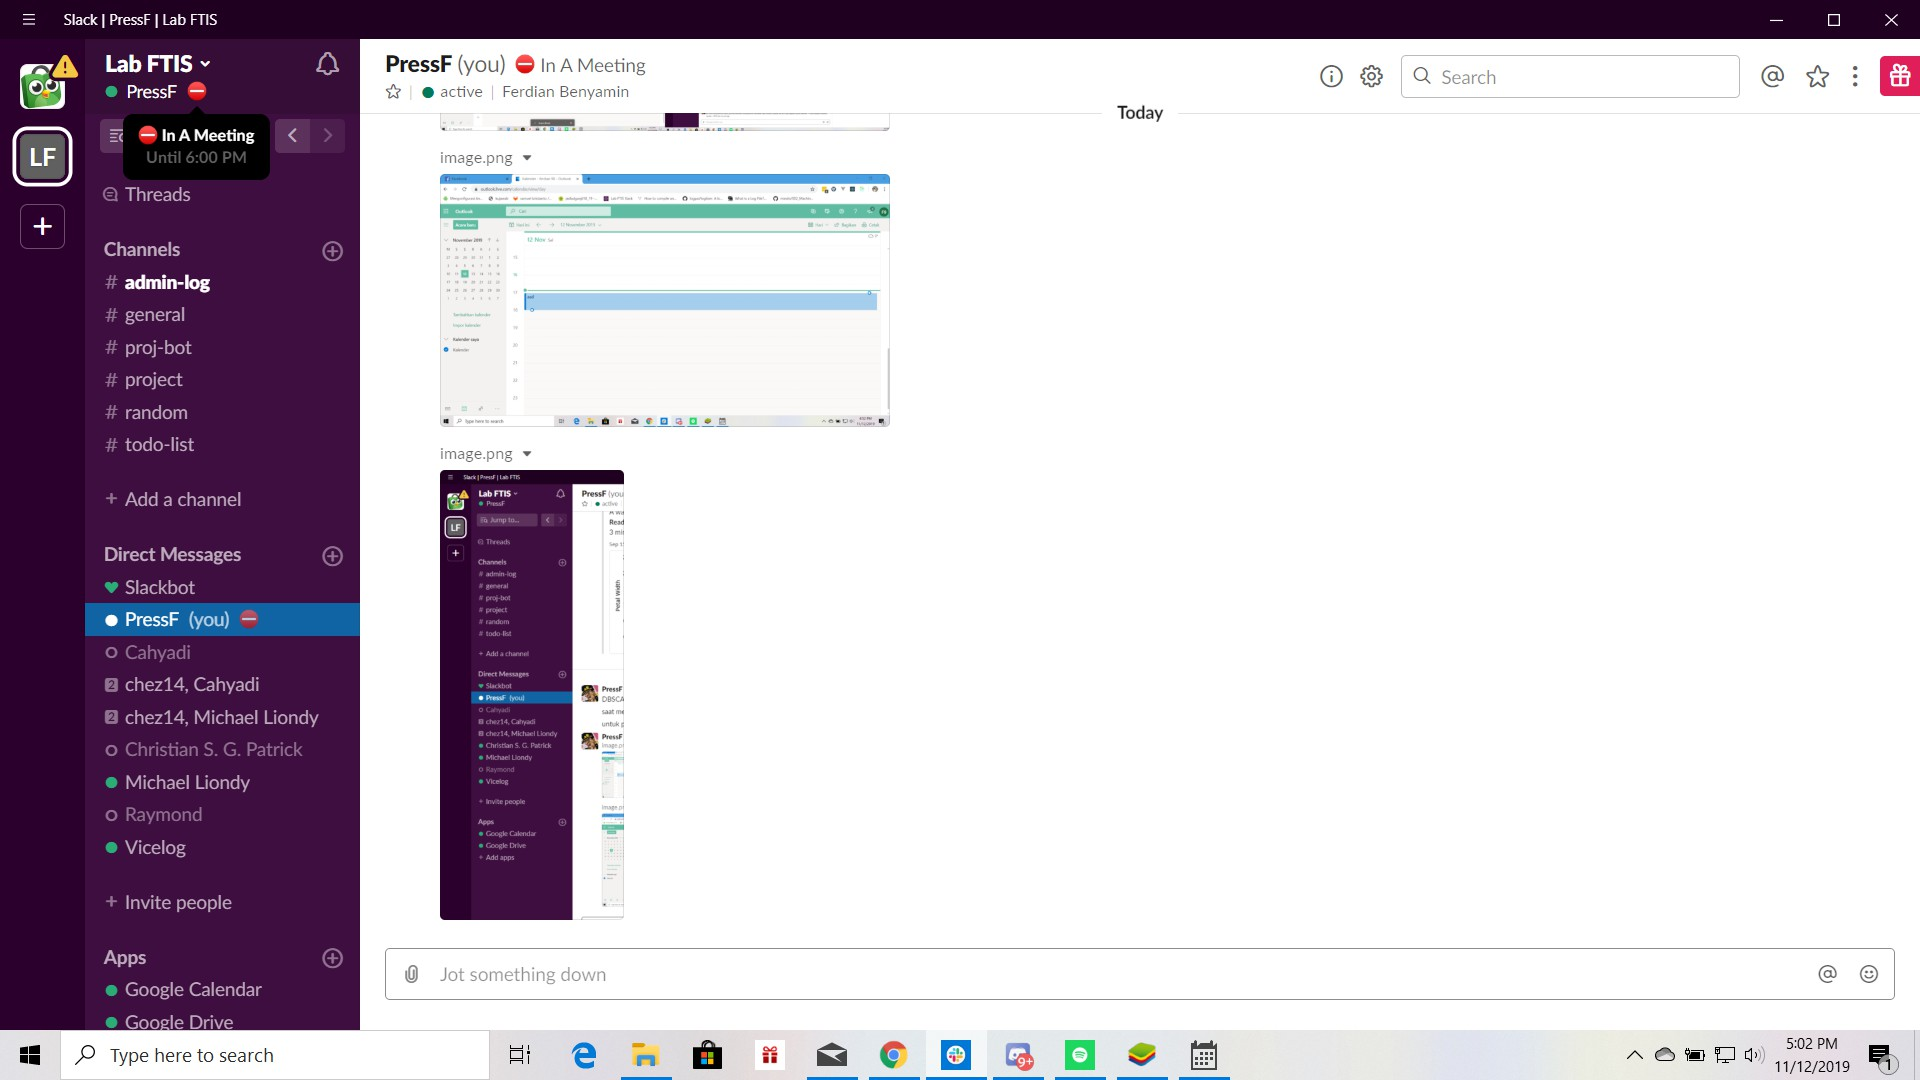
\includegraphics[width=10cm]{./Gambar/PengujianFerdian/Slack_After.jpg}
  \centering
  \caption{Tampilan \textit{Slack} setelah \textit{event} dimulai(Ferdian).}
  \label{fig:slack_after_ferdian}
\end{figure}

Gambar \ref{fig:outlook_ferdian} sampai dengan gambar \ref{fig:slack_after_ferdian} merupakan hasil yang didapat dari hasil pengujian yang dilakukan oleh pengguna yang bernama Ferdian yang merupakan seorang admin di lab FTIS. Pengguna ini menguji perangkat lunak pada \textit{workspace} Lab FTIS. Di gambar \ref{fig:outlook_ferdian} dapat dilihat bahwa pengguna memiliki \textit{event} yang akan berjalan pukul 17.00 dan waktu di komputer nya menunjukkan pukul 16.52. Lalu pada gambar \ref{fig:slack_before_ferdian} dapat terlihat bahwa tidak ada status yang terpasang pada akun pengguna dan pada gambar \ref{fig:slack_after_ferdian} terlihat bahwa sudah ada status yang terpasang pada akun pengguna pada pukul 17.02 dan status itu akan berakhir pada pukul 18.00. 
\clearpage

\begin{figure}[h]
  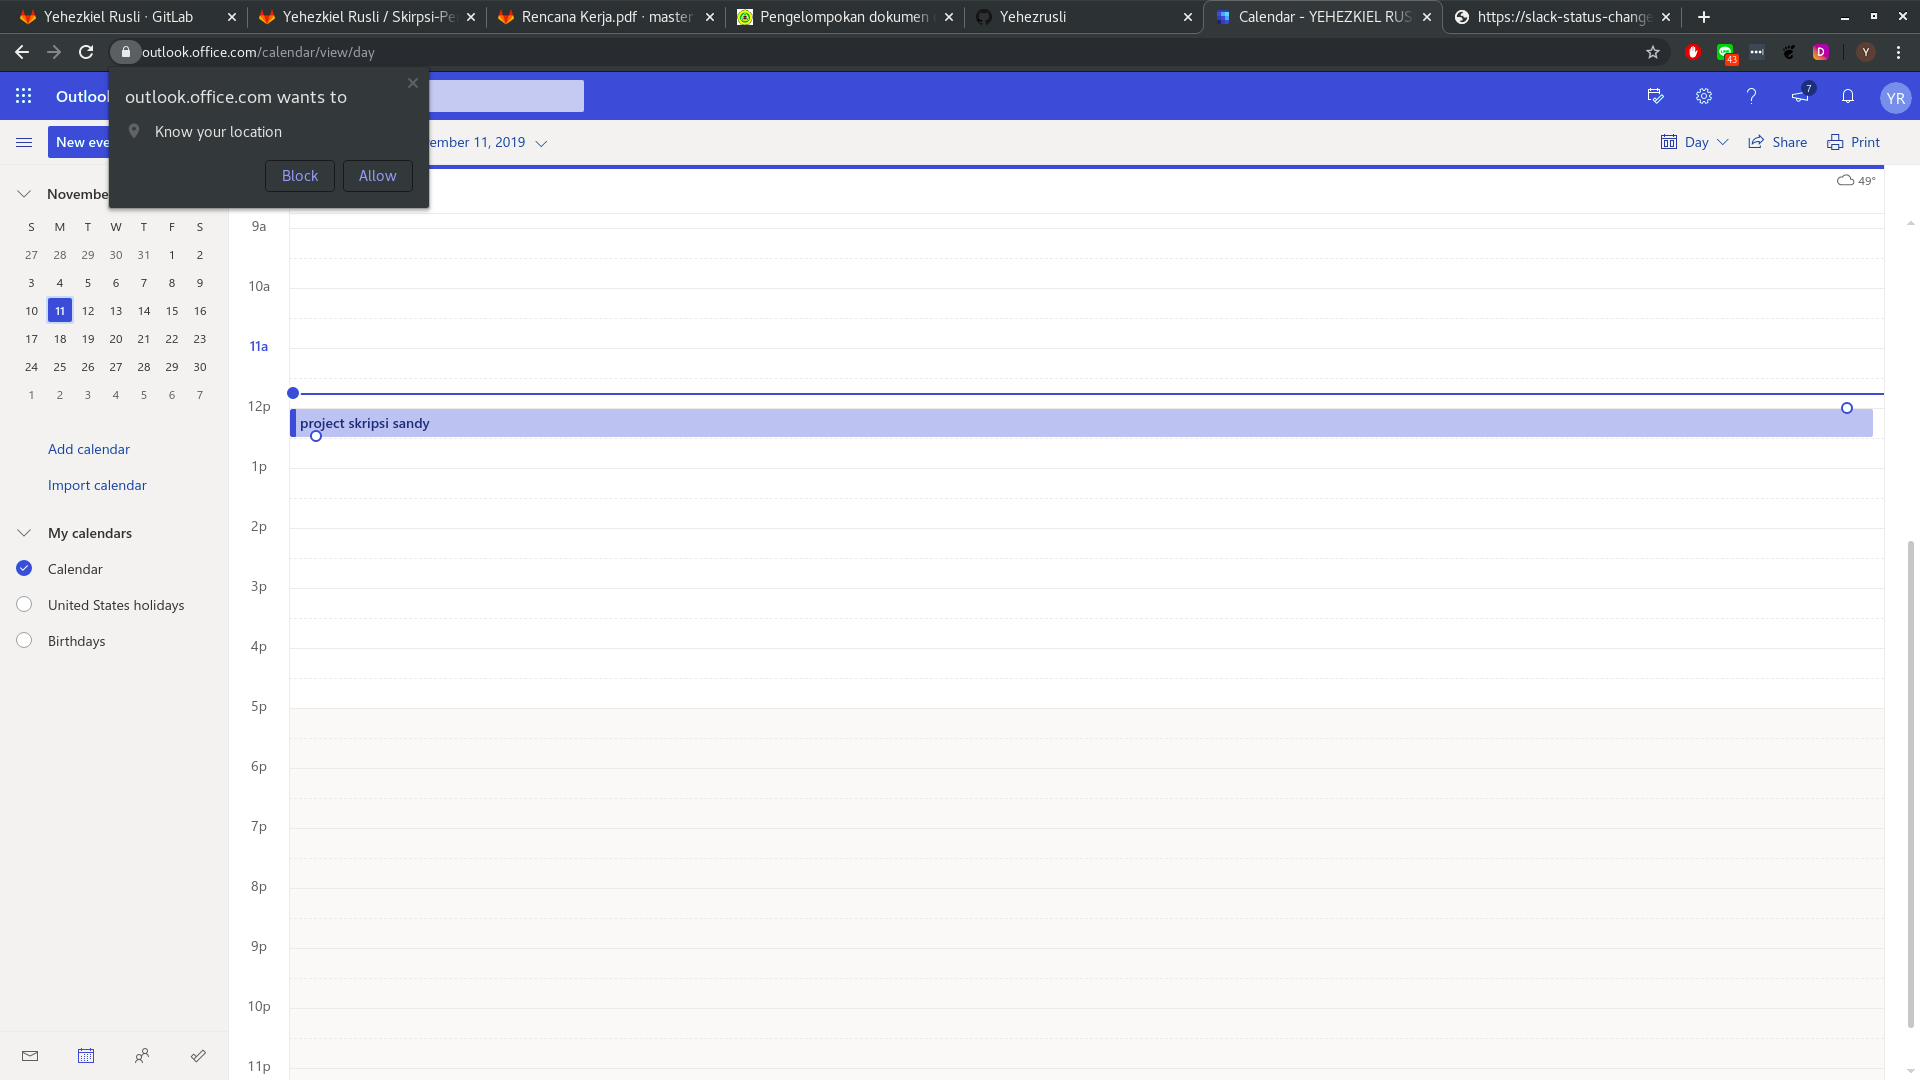
\includegraphics[width=10cm]{./Gambar/PengujianKikil/Outlook.png}
  \centering
  \caption{Tampilan \textit{event} yang dibuat pengguna(Yehezkiel).}
  \label{fig:outlook_kikil}
\end{figure}

\begin{figure}[h]
  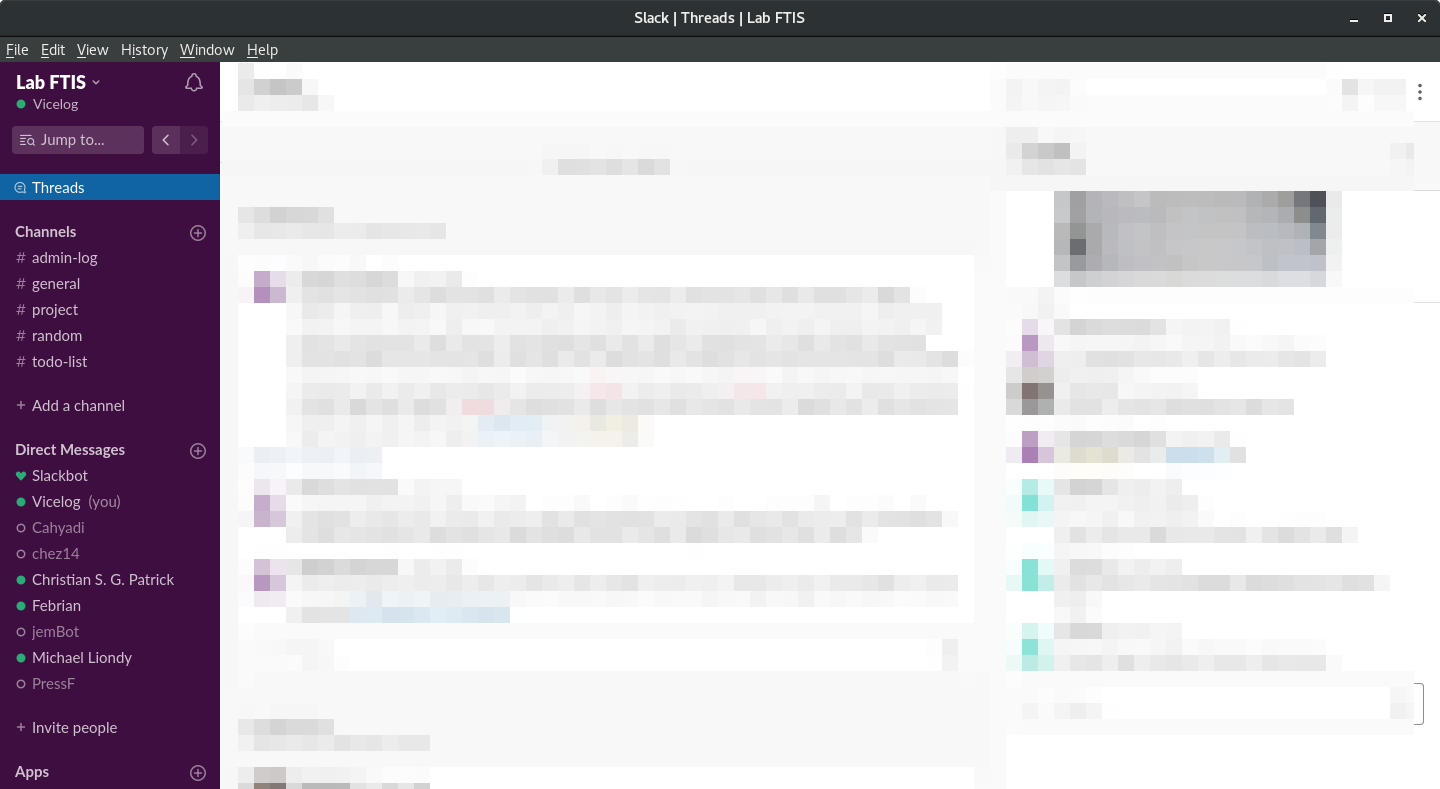
\includegraphics[width=10cm]{./Gambar/PengujianKikil/Slack_Before.png}
  \centering
  \caption{Tampilan \textit{Slack} sebelum \textit{event} dimulai(Yehezkiel).}
  \label{fig:slack_before_kikil}
\end{figure}

\begin{figure}[h]
  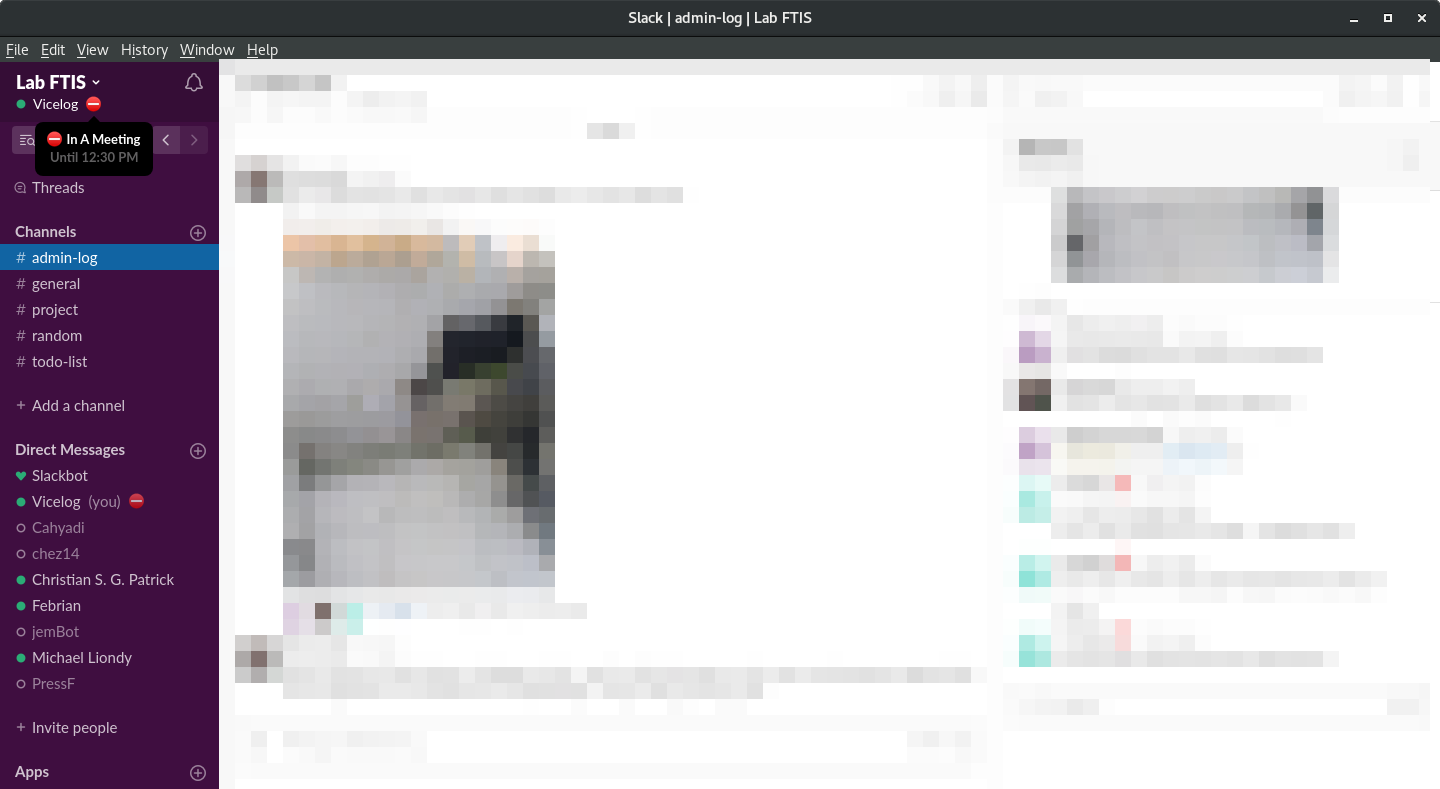
\includegraphics[width=10cm]{./Gambar/PengujianKikil/Slack_After.png}
  \centering
  \caption{Tampilan \textit{Slack} setelah \textit{event} dimulai(Yehezkiel).}
  \label{fig:slack_after_kikil}
\end{figure}

Dari gambar \ref{fig:outlook_kikil} sampai dengan gambar \ref{fig:slack_after_kikil} merupakan bukti yang didapatkan oleh pengguna yang bernama Yehezkiel yang merupakan seorang admin di lab FTIS pada saat pengujian perangkat lunak ini. Pengguna ini menguji di \textit{workspace} Lab FTIS. Pada gambar \ref{fig:outlook_kikil} terdapat sebuah \textit{event} yang akan dimulai pada pukul 12.00 dan pada gambar \ref{fig:slack_before_kikil} belum terdapat adanya status yang terpasang pada akun pengguna. Lalu pada gambar \ref{fig:slack_after_kikil} dapat terlihat bahwa sudah ada status yang terpasang dan akan berakhir pada pukul 12.30. 
\clearpage

\begin{figure}[h]
  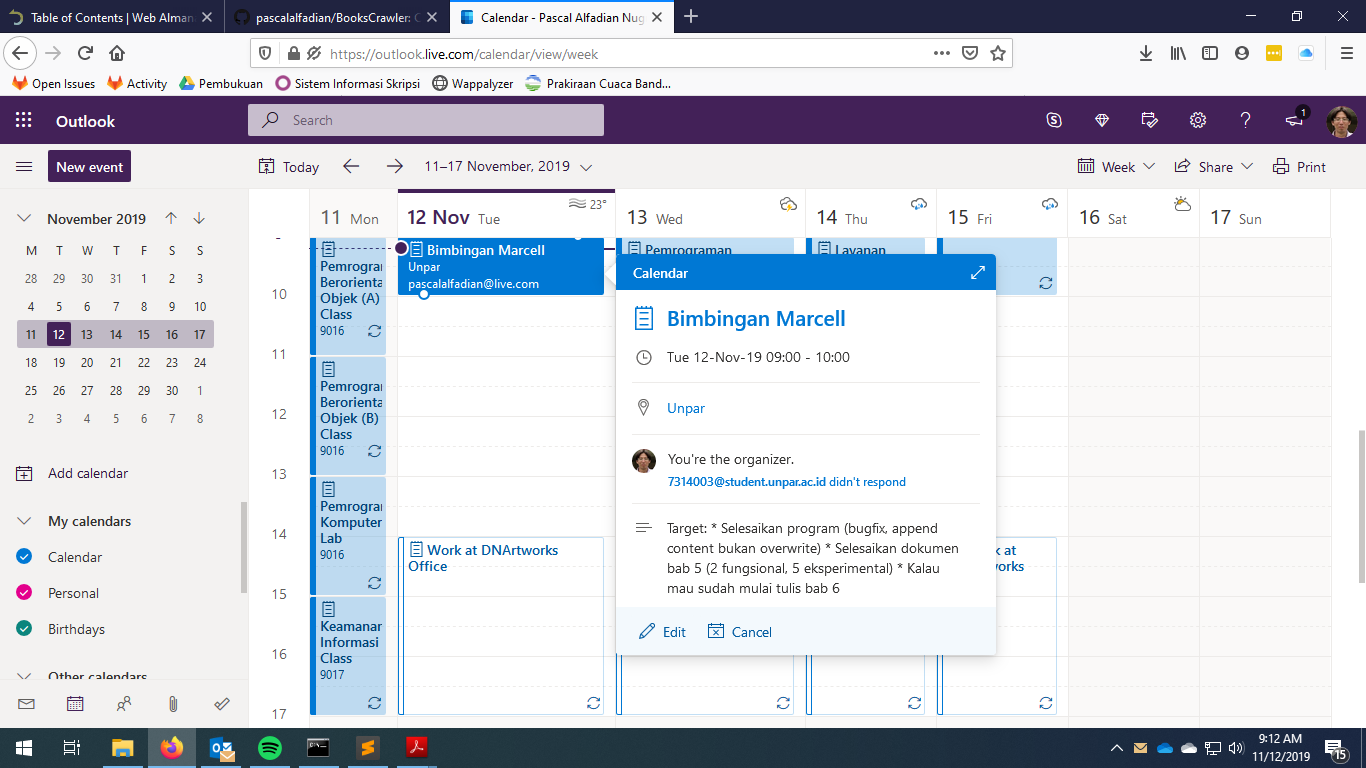
\includegraphics[width=10cm]{./Gambar/PengujianPaPascal/Outlook.png}
  \centering
  \caption{Tampilan \textit{event} yang dibuat pengguna(Pascal).}
  \label{fig:outlook_pascal}
\end{figure}

\begin{figure}[h]
  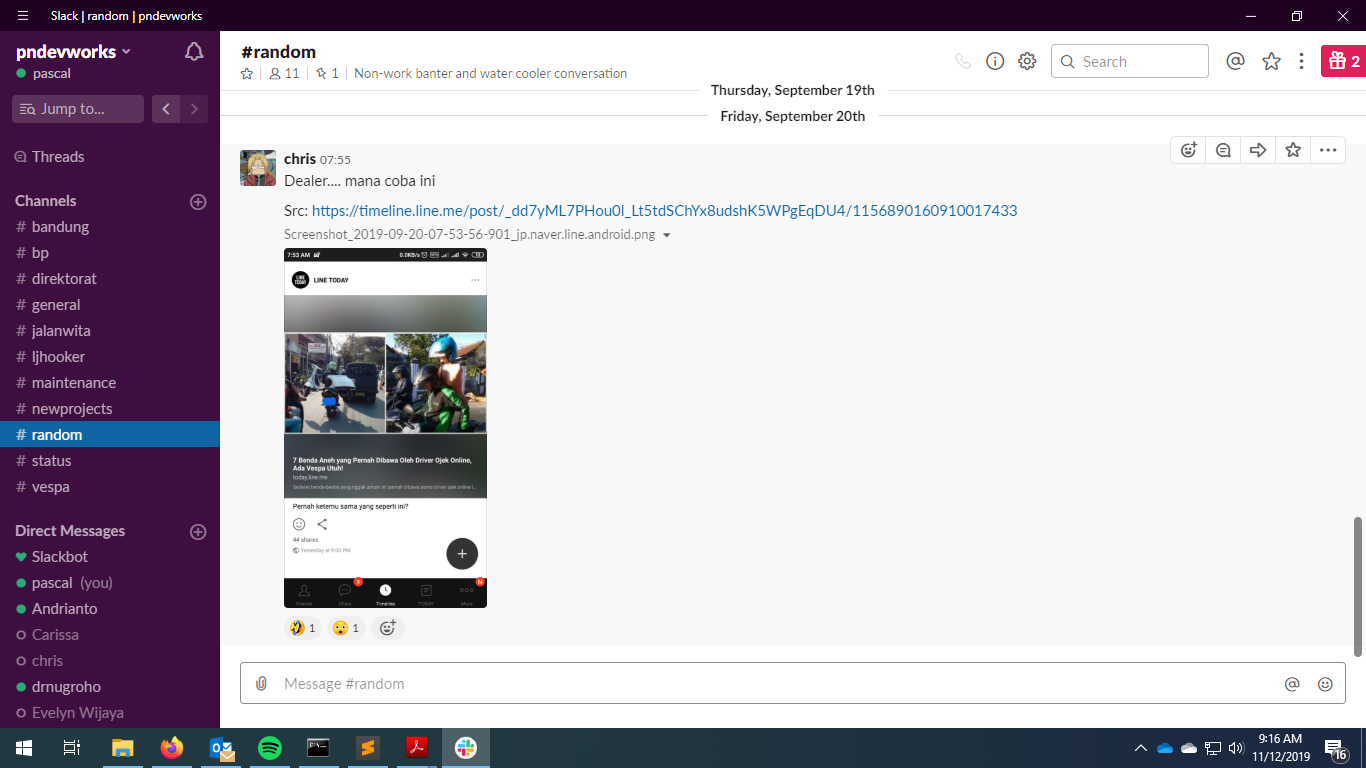
\includegraphics[width=10cm]{./Gambar/PengujianPaPascal/Slack_After_Authorize_PL.png}
  \centering
  \caption{Tampilan \textit{Slack} setelah mengizinkan perangkat lunak kepada \textit{workspace Slack}(Pascal).}
  \label{fig:slack_after_auth_pascal}
\end{figure}

\begin{figure}[h]
  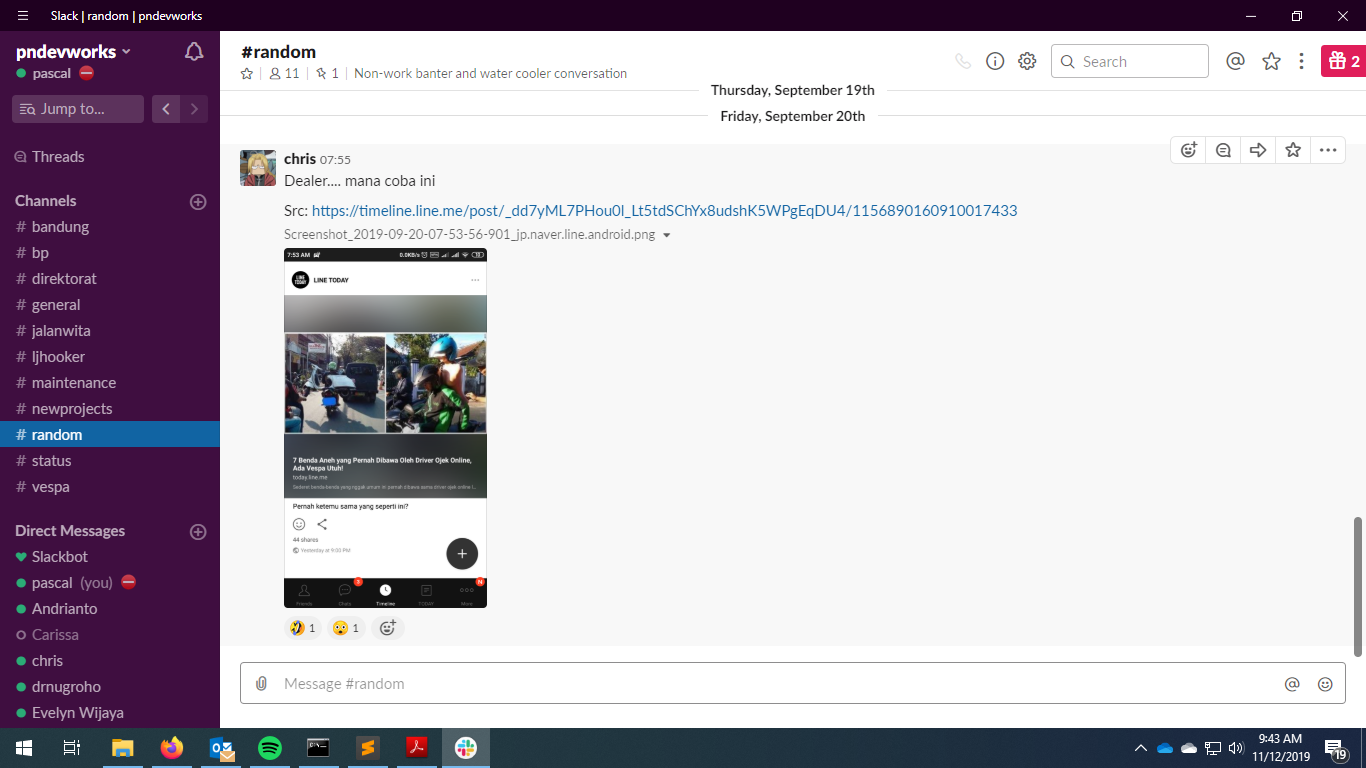
\includegraphics[width=10cm]{./Gambar/PengujianPaPascal/Slack_After.png}
  \centering
  \caption{Tampilan \textit{Slack} setelah \textit{event} dimulai(Pascal).}
  \label{fig:slack_after_pascal}
\end{figure}

\begin{figure}[h]
  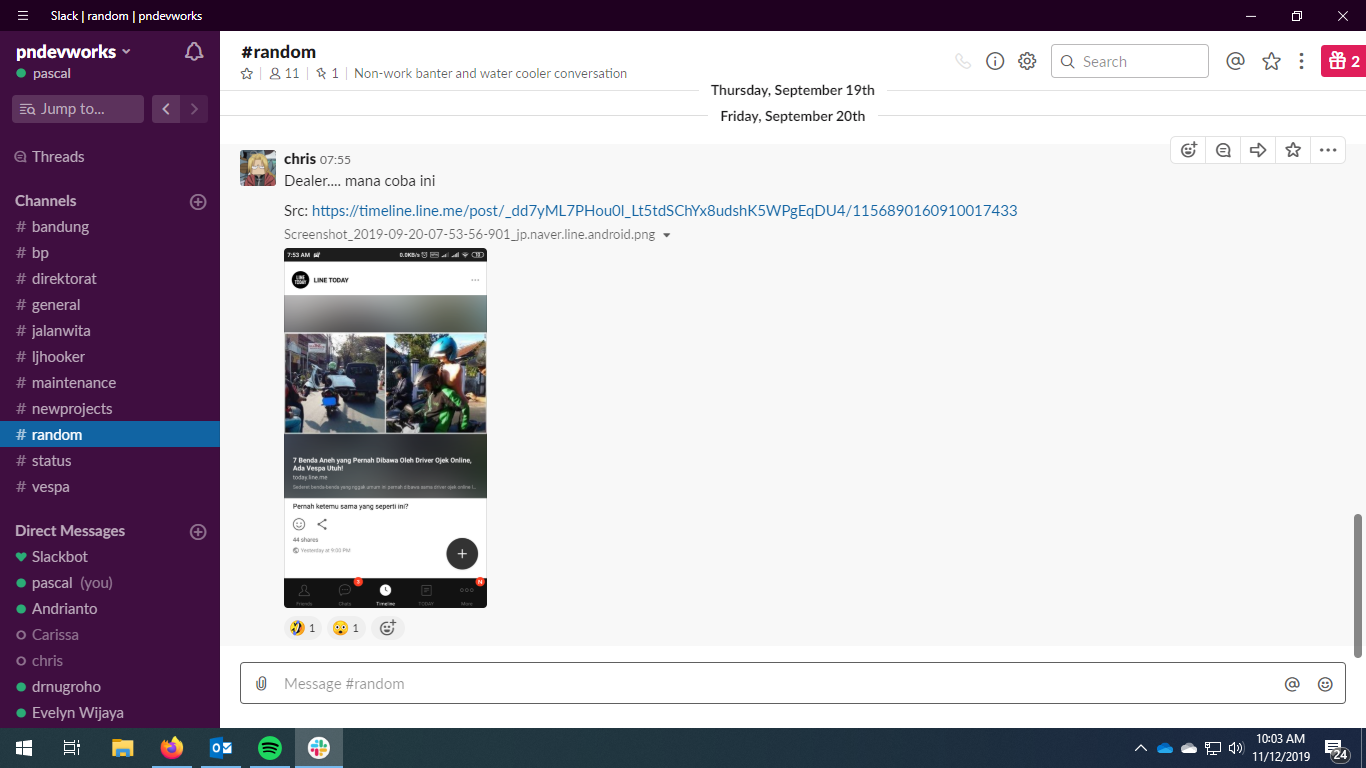
\includegraphics[width=10cm]{./Gambar/PengujianPaPascal/Slack_After_Event_End.png}
  \centering
  \caption{Tampilan \textit{Slack} setelah \textit{event} berakhir(Pascal).}
  \label{fig:slack_after_event_end_pascal}
\end{figure}

Dari gambar \ref{fig:outlook_pascal} sampai \ref{fig:slack_after_event_end_pascal} merupakan hasil dari pengujian yang dilakukan oleh pengguna bernama Pascal yang mencoba perangkat lunak di \textit{workspace} pndevworks. Pada gambar \ref{fig:outlook_pascal} terlihat ada \textit{event} yang sedang berjalan yaitu dimulai dari pukul 09.00 sampai 10.00. Tetapi pengguna baru selesai menjalankan perangkat lunak yang dibangun dan berhasil memberikan izin pada pukul 09.13 yang bisa dilihat pada gambar \ref{fig:slack_after_auth_pascal} bahwa pada pukul 09.16 status masih belum berubah. Pada pukul 09.43 status sudah berubah seperti gambar \ref{fig:slack_after_pascal} dan status sudah hilang pada pukul 10.03 seperti pada gambar \ref{fig:slack_after_event_end_pascal}.  

\clearpage

\begin{figure}[h]
  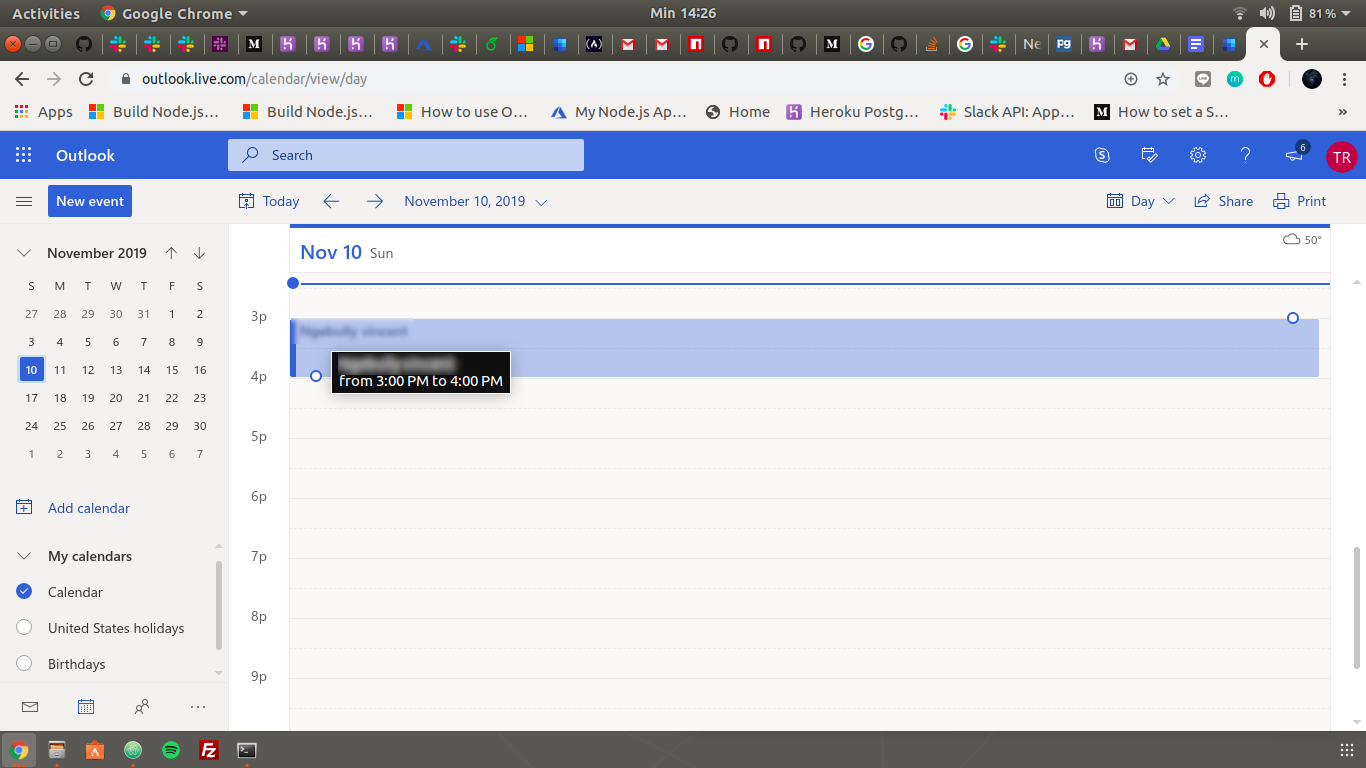
\includegraphics[width=10cm]{./Gambar/PengujianTedi/Outlook.png}
  \centering
  \caption{Tampilan \textit{event} yang dibuat pengguna(Tedi).}
  \label{fig:outlook_tedi}
\end{figure}

\begin{figure}[h]
  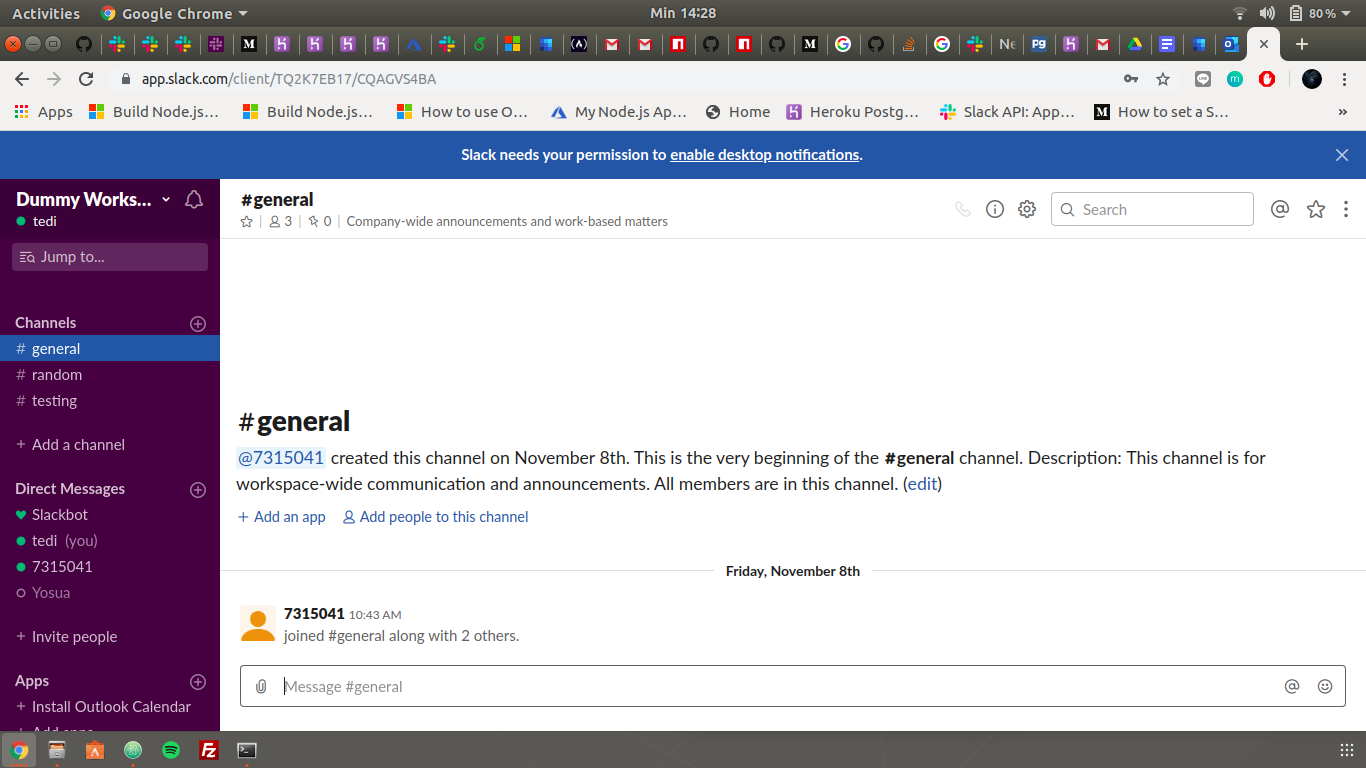
\includegraphics[width=10cm]{./Gambar/PengujianTedi/Slack_Before.png}
  \centering
  \caption{Tampilan \textit{Slack} sebelum \textit{event} dimulai(Tedi).}
  \label{fig:slack_before_tedi}
\end{figure}

\begin{figure}[h]
  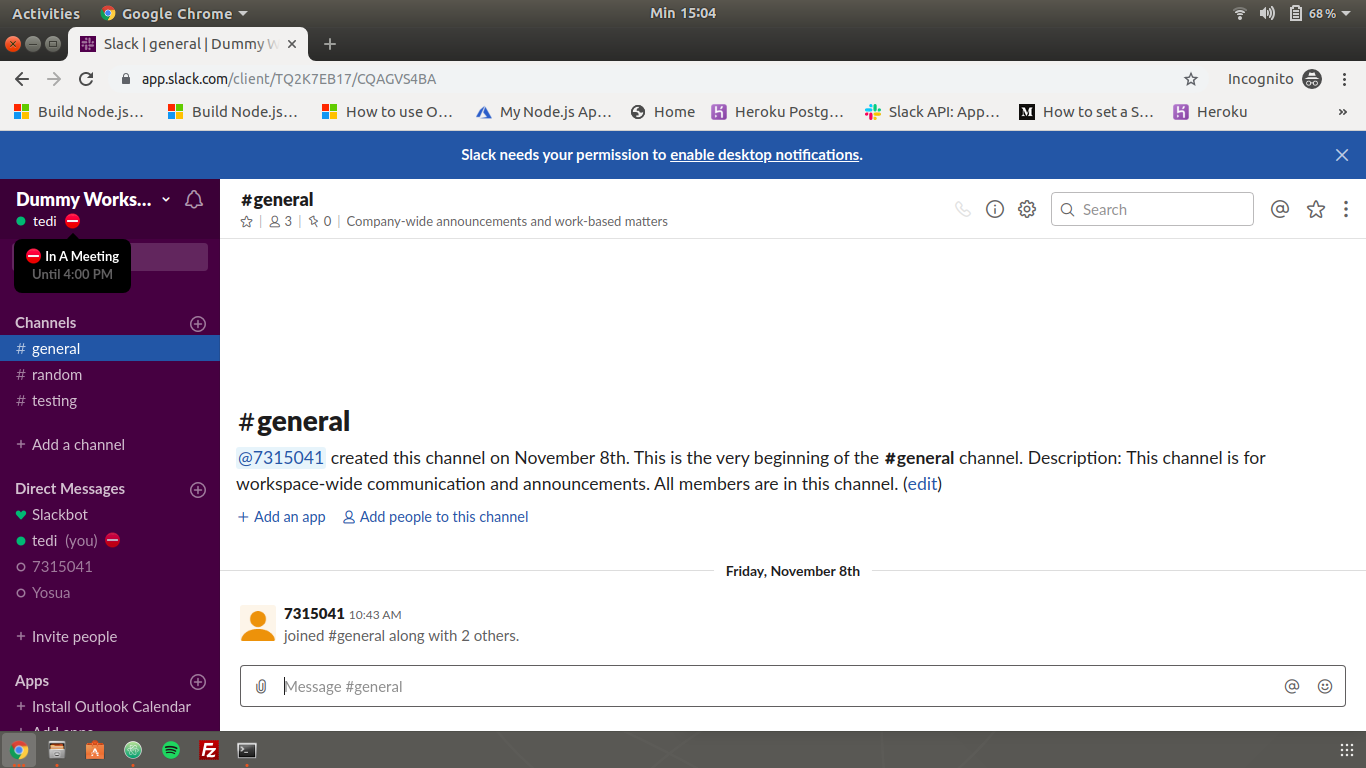
\includegraphics[width=10cm]{./Gambar/PengujianTedi/Slack_After.png}
  \centering
  \caption{Tampilan \textit{Slack} setelah \textit{event} dimulai(Tedi).}
  \label{fig:slack_after_tedi}
\end{figure}

Dari gambar \ref{fig:outlook_tedi} sampai dengan gambar \ref{fig:slack_after_tedi} merupakan hasil pengujian dari pengguna yang bernama Tedi. Pengguna ini mencoba di \textit{workspace} yang bernama Dummy Workspace. Pada gambar \ref{fig:outlook_tedi} terdapat \textit{event} yang terdaftar yang dimulai pada pukul 15.00 dan pada gambar \ref{fig:slack_before_tedi} terlihat waktu pada komputer menunjukkan pukul 14.28 dan belum terdapat status yang terpasang pada akun pengguna. Pada gambar \ref{fig:slack_after_tedi} menunjukkan pada pukul 15.04 pada komputer, di akun pengguna sudah terpasang status yang statusnya akan berakhir pada pukul 16.00. 
\clearpage

\begin{figure}[h]
  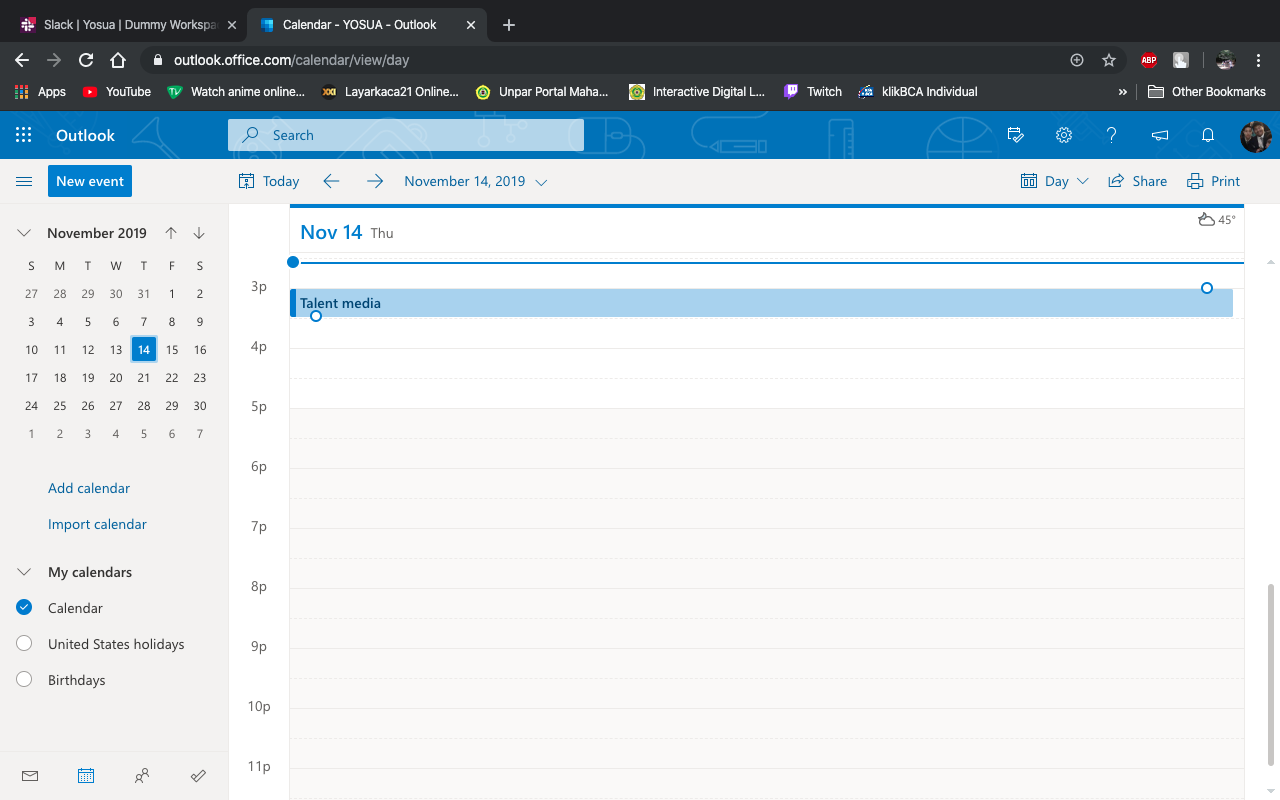
\includegraphics[width=10cm]{./Gambar/PengujianYosua/Outlook.png}
  \centering
  \caption{Tampilan \textit{event} yang dibuat pengguna(Yosua).}
  \label{fig:outlook_yosua}
\end{figure}

\begin{figure}[h]
  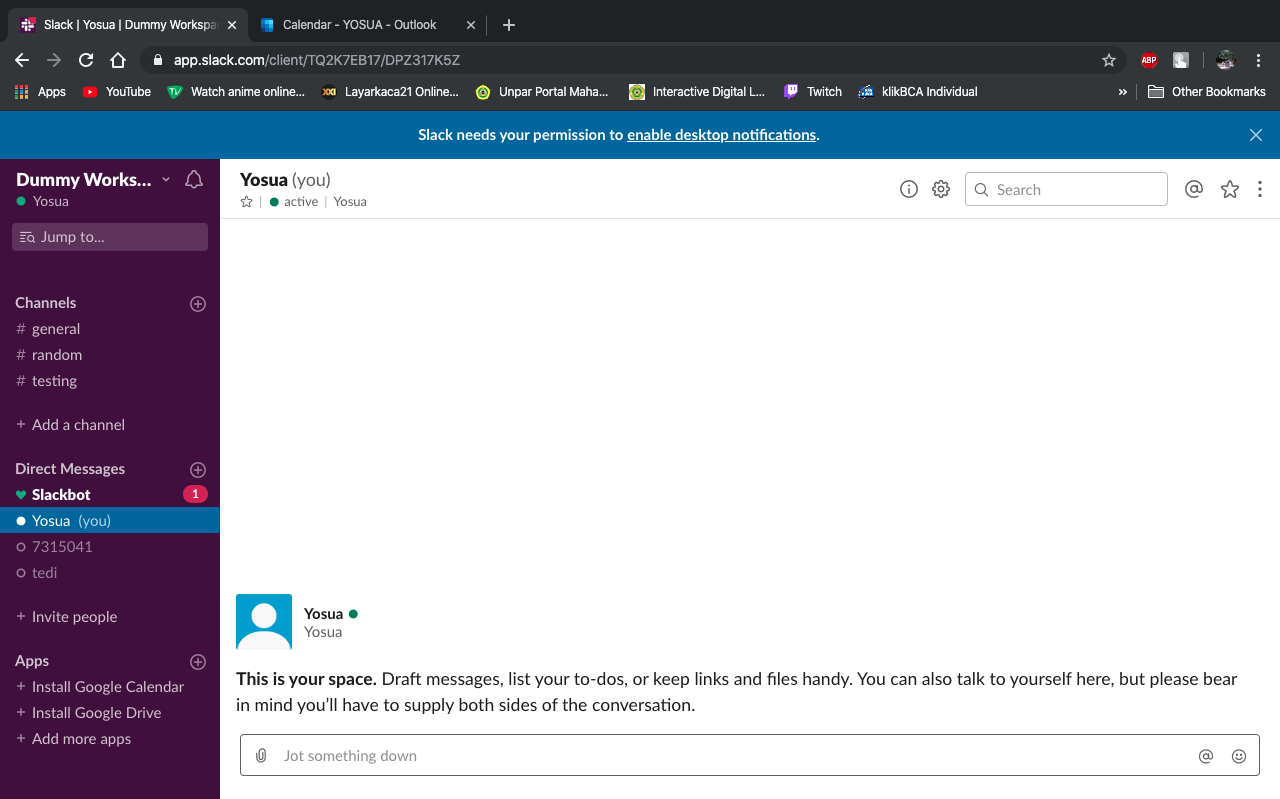
\includegraphics[width=10cm]{./Gambar/PengujianYosua/Slack_Before.png}
  \centering
  \caption{Tampilan \textit{Slack} sebelum \textit{event} dimulai(Yosua).}
  \label{fig:slack_before_yosua}
\end{figure}

\begin{figure}[h]
  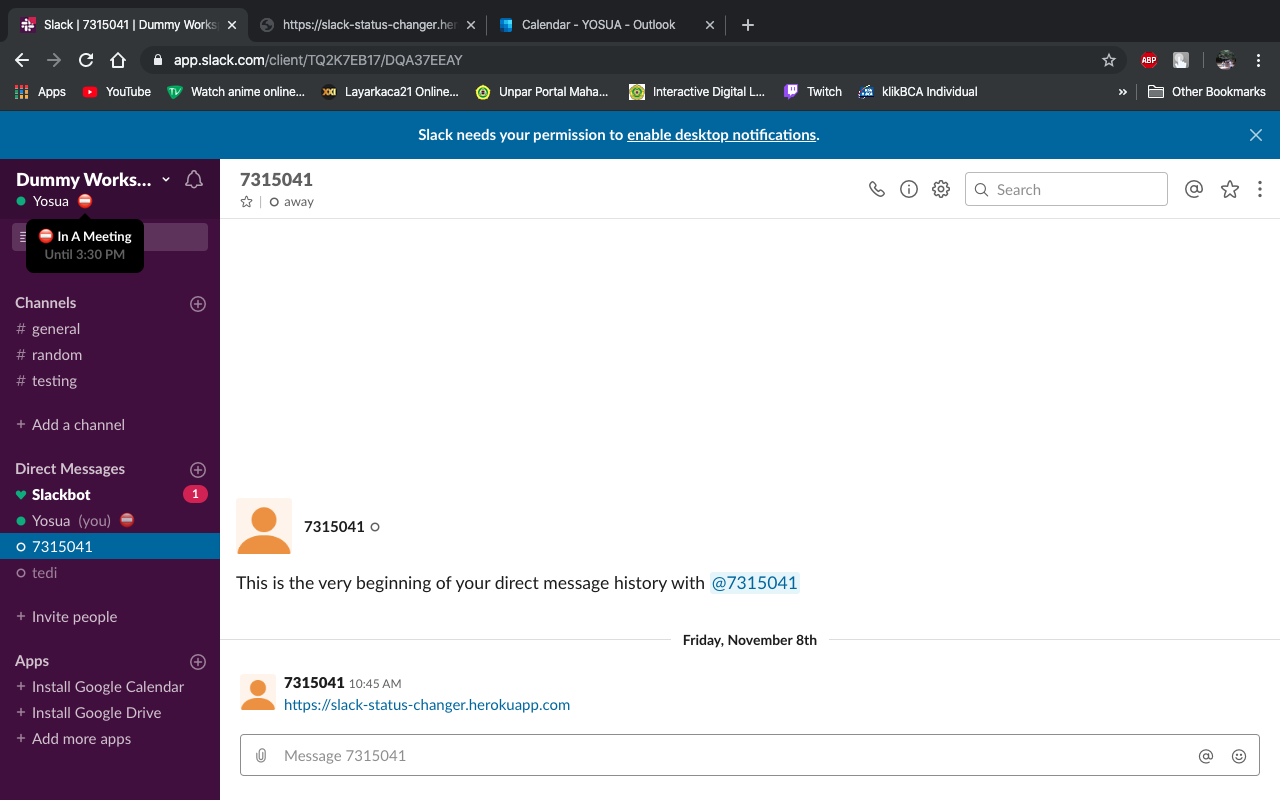
\includegraphics[width=10cm]{./Gambar/PengujianYosua/Slack_After.png}
  \centering
  \caption{Tampilan \textit{Slack} setelah \textit{event} dimulai(Yosua).}
  \label{fig:slack_after_yosua}
\end{figure}

Pada gambar \ref{fig:outlook_yosua} sampai gambar \ref{fig:slack_after_yosua} merupakan hasil yang didapatkan dari pengujian oleh pengguna yang bernama Yosua. Pengguna ini mencoba perangkat lunak ini di \textit{workspace} Dummy Workspace. Pada gambar \ref{fig:outlook_yosua} terdapat \textit{event} yang dimulai pada pukul 15.00 dan pada gambar \ref{fig:slack_before_yosua} status pengguna masih kosong. Pada gambar \ref{fig:slack_after_yosua} sudah terlihat ada status dan status itu berakhir pada pukul 15.30. 
\clearpage

\subsubsection{Kesimpulan dari Pengujian}
Pada pengujian yang sudah dilakukan oleh beberapa pengguna yang terlibat menyatakan bahwa perangkat lunak menjalankan fungsinya untuk mengganti status pada saat ada \textit{event} dan menggantinya kembali jika \textit{event} sudah berhasil dengan baik. Hanya saja terdapat perbedaan jeda saat mengubah status sehingga tidak tepat pada saat \textit{event} dimulai maka status langsung berubah. Hal ini dikarenakan adanya proses yang dilakukan setiap kali memanggil fungsi yang dijalankan kurang lebih 2 menit sehingga mempengaruhi jadwal iterasi dari \textit{Heroku Scheduler} yang selanjutnya. 